\documentclass[]{article}
\usepackage{lmodern}
\usepackage{amssymb,amsmath}
\usepackage{ifxetex,ifluatex}
\usepackage{fixltx2e} % provides \textsubscript
\ifnum 0\ifxetex 1\fi\ifluatex 1\fi=0 % if pdftex
  \usepackage[T1]{fontenc}
  \usepackage[utf8]{inputenc}
\else % if luatex or xelatex
  \ifxetex
    \usepackage{mathspec}
  \else
    \usepackage{fontspec}
  \fi
  \defaultfontfeatures{Ligatures=TeX,Scale=MatchLowercase}
\fi
% use upquote if available, for straight quotes in verbatim environments
\IfFileExists{upquote.sty}{\usepackage{upquote}}{}
% use microtype if available
\IfFileExists{microtype.sty}{%
\usepackage{microtype}
\UseMicrotypeSet[protrusion]{basicmath} % disable protrusion for tt fonts
}{}
\usepackage[margin=1in]{geometry}
\usepackage{hyperref}
\hypersetup{unicode=true,
            pdftitle={IEO\_PROJECT},
            pdfauthor={Javier Sánchez Utgés},
            pdfborder={0 0 0},
            breaklinks=true}
\urlstyle{same}  % don't use monospace font for urls
\usepackage{color}
\usepackage{fancyvrb}
\newcommand{\VerbBar}{|}
\newcommand{\VERB}{\Verb[commandchars=\\\{\}]}
\DefineVerbatimEnvironment{Highlighting}{Verbatim}{commandchars=\\\{\}}
% Add ',fontsize=\small' for more characters per line
\usepackage{framed}
\definecolor{shadecolor}{RGB}{248,248,248}
\newenvironment{Shaded}{\begin{snugshade}}{\end{snugshade}}
\newcommand{\KeywordTok}[1]{\textcolor[rgb]{0.13,0.29,0.53}{\textbf{{#1}}}}
\newcommand{\DataTypeTok}[1]{\textcolor[rgb]{0.13,0.29,0.53}{{#1}}}
\newcommand{\DecValTok}[1]{\textcolor[rgb]{0.00,0.00,0.81}{{#1}}}
\newcommand{\BaseNTok}[1]{\textcolor[rgb]{0.00,0.00,0.81}{{#1}}}
\newcommand{\FloatTok}[1]{\textcolor[rgb]{0.00,0.00,0.81}{{#1}}}
\newcommand{\ConstantTok}[1]{\textcolor[rgb]{0.00,0.00,0.00}{{#1}}}
\newcommand{\CharTok}[1]{\textcolor[rgb]{0.31,0.60,0.02}{{#1}}}
\newcommand{\SpecialCharTok}[1]{\textcolor[rgb]{0.00,0.00,0.00}{{#1}}}
\newcommand{\StringTok}[1]{\textcolor[rgb]{0.31,0.60,0.02}{{#1}}}
\newcommand{\VerbatimStringTok}[1]{\textcolor[rgb]{0.31,0.60,0.02}{{#1}}}
\newcommand{\SpecialStringTok}[1]{\textcolor[rgb]{0.31,0.60,0.02}{{#1}}}
\newcommand{\ImportTok}[1]{{#1}}
\newcommand{\CommentTok}[1]{\textcolor[rgb]{0.56,0.35,0.01}{\textit{{#1}}}}
\newcommand{\DocumentationTok}[1]{\textcolor[rgb]{0.56,0.35,0.01}{\textbf{\textit{{#1}}}}}
\newcommand{\AnnotationTok}[1]{\textcolor[rgb]{0.56,0.35,0.01}{\textbf{\textit{{#1}}}}}
\newcommand{\CommentVarTok}[1]{\textcolor[rgb]{0.56,0.35,0.01}{\textbf{\textit{{#1}}}}}
\newcommand{\OtherTok}[1]{\textcolor[rgb]{0.56,0.35,0.01}{{#1}}}
\newcommand{\FunctionTok}[1]{\textcolor[rgb]{0.00,0.00,0.00}{{#1}}}
\newcommand{\VariableTok}[1]{\textcolor[rgb]{0.00,0.00,0.00}{{#1}}}
\newcommand{\ControlFlowTok}[1]{\textcolor[rgb]{0.13,0.29,0.53}{\textbf{{#1}}}}
\newcommand{\OperatorTok}[1]{\textcolor[rgb]{0.81,0.36,0.00}{\textbf{{#1}}}}
\newcommand{\BuiltInTok}[1]{{#1}}
\newcommand{\ExtensionTok}[1]{{#1}}
\newcommand{\PreprocessorTok}[1]{\textcolor[rgb]{0.56,0.35,0.01}{\textit{{#1}}}}
\newcommand{\AttributeTok}[1]{\textcolor[rgb]{0.77,0.63,0.00}{{#1}}}
\newcommand{\RegionMarkerTok}[1]{{#1}}
\newcommand{\InformationTok}[1]{\textcolor[rgb]{0.56,0.35,0.01}{\textbf{\textit{{#1}}}}}
\newcommand{\WarningTok}[1]{\textcolor[rgb]{0.56,0.35,0.01}{\textbf{\textit{{#1}}}}}
\newcommand{\AlertTok}[1]{\textcolor[rgb]{0.94,0.16,0.16}{{#1}}}
\newcommand{\ErrorTok}[1]{\textcolor[rgb]{0.64,0.00,0.00}{\textbf{{#1}}}}
\newcommand{\NormalTok}[1]{{#1}}
\usepackage{graphicx,grffile}
\makeatletter
\def\maxwidth{\ifdim\Gin@nat@width>\linewidth\linewidth\else\Gin@nat@width\fi}
\def\maxheight{\ifdim\Gin@nat@height>\textheight\textheight\else\Gin@nat@height\fi}
\makeatother
% Scale images if necessary, so that they will not overflow the page
% margins by default, and it is still possible to overwrite the defaults
% using explicit options in \includegraphics[width, height, ...]{}
\setkeys{Gin}{width=\maxwidth,height=\maxheight,keepaspectratio}
\IfFileExists{parskip.sty}{%
\usepackage{parskip}
}{% else
\setlength{\parindent}{0pt}
\setlength{\parskip}{6pt plus 2pt minus 1pt}
}
\setlength{\emergencystretch}{3em}  % prevent overfull lines
\providecommand{\tightlist}{%
  \setlength{\itemsep}{0pt}\setlength{\parskip}{0pt}}
\setcounter{secnumdepth}{0}
% Redefines (sub)paragraphs to behave more like sections
\ifx\paragraph\undefined\else
\let\oldparagraph\paragraph
\renewcommand{\paragraph}[1]{\oldparagraph{#1}\mbox{}}
\fi
\ifx\subparagraph\undefined\else
\let\oldsubparagraph\subparagraph
\renewcommand{\subparagraph}[1]{\oldsubparagraph{#1}\mbox{}}
\fi

%%% Use protect on footnotes to avoid problems with footnotes in titles
\let\rmarkdownfootnote\footnote%
\def\footnote{\protect\rmarkdownfootnote}

%%% Change title format to be more compact
\usepackage{titling}

% Create subtitle command for use in maketitle
\providecommand{\subtitle}[1]{
  \posttitle{
    \begin{center}\large#1\end{center}
    }
}

\setlength{\droptitle}{-2em}

  \title{IEO\_PROJECT}
    \pretitle{\vspace{\droptitle}\centering\huge}
  \posttitle{\par}
    \author{Javier Sánchez Utgés}
    \preauthor{\centering\large\emph}
  \postauthor{\par}
      \predate{\centering\large\emph}
  \postdate{\par}
    \date{30 de abril de 2019}


\begin{document}
\maketitle

\section{Analysis of TCGA RNA-seq dataset of kidney renal clear cell
carcinoma}\label{analysis-of-tcga-rna-seq-dataset-of-kidney-renal-clear-cell-carcinoma}

This is an R Markdown document that will show all the steps of the
analysis of TCGA RNA-seq dataset of kidney renal clear cell carcinoma.

\subsection{1. Introduction}\label{introduction}

\subsection{2. Quality analysis}\label{quality-analysis}

\subsubsection{2.1. Data import}\label{data-import}

First, we import the dataset and store it in a
\texttt{SummarizedExperiment} object, named \texttt{se}. This kind of
object has genes on its rows and samples on its columns, 20,115 genes
and 614 samples in our case. Both of these entities have their own
associated metadata, i.e., gene symbol, lenght and GC content for genes.
For samples, there are more than 500 more fields, for instance type,
gender and race.

\begin{verbatim}
## Warning: package 'SummarizedExperiment' was built under R version 3.4.3
\end{verbatim}

\begin{verbatim}
## Loading required package: GenomicRanges
\end{verbatim}

\begin{verbatim}
## Warning: package 'GenomicRanges' was built under R version 3.4.4
\end{verbatim}

\begin{verbatim}
## Loading required package: stats4
\end{verbatim}

\begin{verbatim}
## Loading required package: BiocGenerics
\end{verbatim}

\begin{verbatim}
## Warning: package 'BiocGenerics' was built under R version 3.4.2
\end{verbatim}

\begin{verbatim}
## Loading required package: parallel
\end{verbatim}

\begin{verbatim}
## 
## Attaching package: 'BiocGenerics'
\end{verbatim}

\begin{verbatim}
## The following objects are masked from 'package:parallel':
## 
##     clusterApply, clusterApplyLB, clusterCall, clusterEvalQ,
##     clusterExport, clusterMap, parApply, parCapply, parLapply,
##     parLapplyLB, parRapply, parSapply, parSapplyLB
\end{verbatim}

\begin{verbatim}
## The following objects are masked from 'package:stats':
## 
##     IQR, mad, sd, var, xtabs
\end{verbatim}

\begin{verbatim}
## The following objects are masked from 'package:base':
## 
##     anyDuplicated, append, as.data.frame, cbind, colMeans,
##     colnames, colSums, do.call, duplicated, eval, evalq, Filter,
##     Find, get, grep, grepl, intersect, is.unsorted, lapply,
##     lengths, Map, mapply, match, mget, order, paste, pmax,
##     pmax.int, pmin, pmin.int, Position, rank, rbind, Reduce,
##     rowMeans, rownames, rowSums, sapply, setdiff, sort, table,
##     tapply, union, unique, unsplit, which, which.max, which.min
\end{verbatim}

\begin{verbatim}
## Loading required package: S4Vectors
\end{verbatim}

\begin{verbatim}
## Warning: package 'S4Vectors' was built under R version 3.4.2
\end{verbatim}

\begin{verbatim}
## 
## Attaching package: 'S4Vectors'
\end{verbatim}

\begin{verbatim}
## The following object is masked from 'package:base':
## 
##     expand.grid
\end{verbatim}

\begin{verbatim}
## Loading required package: IRanges
\end{verbatim}

\begin{verbatim}
## Warning: package 'IRanges' was built under R version 3.4.2
\end{verbatim}

\begin{verbatim}
## Loading required package: GenomeInfoDb
\end{verbatim}

\begin{verbatim}
## Warning: package 'GenomeInfoDb' was built under R version 3.4.2
\end{verbatim}

\begin{verbatim}
## Loading required package: Biobase
\end{verbatim}

\begin{verbatim}
## Warning: package 'Biobase' was built under R version 3.4.2
\end{verbatim}

\begin{verbatim}
## Welcome to Bioconductor
## 
##     Vignettes contain introductory material; view with
##     'browseVignettes()'. To cite Bioconductor, see
##     'citation("Biobase")', and for packages 'citation("pkgname")'.
\end{verbatim}

\begin{verbatim}
## Loading required package: DelayedArray
\end{verbatim}

\begin{verbatim}
## Warning: package 'DelayedArray' was built under R version 3.4.2
\end{verbatim}

\begin{verbatim}
## Loading required package: matrixStats
\end{verbatim}

\begin{verbatim}
## Warning: package 'matrixStats' was built under R version 3.4.4
\end{verbatim}

\begin{verbatim}
## 
## Attaching package: 'matrixStats'
\end{verbatim}

\begin{verbatim}
## The following objects are masked from 'package:Biobase':
## 
##     anyMissing, rowMedians
\end{verbatim}

\begin{verbatim}
## 
## Attaching package: 'DelayedArray'
\end{verbatim}

\begin{verbatim}
## The following objects are masked from 'package:matrixStats':
## 
##     colMaxs, colMins, colRanges, rowMaxs, rowMins, rowRanges
\end{verbatim}

\begin{verbatim}
## The following object is masked from 'package:base':
## 
##     apply
\end{verbatim}

\begin{verbatim}
## class: RangedSummarizedExperiment 
## dim: 20115 614 
## metadata(5): experimentData annotation cancerTypeCode
##   cancerTypeDescription objectCreationDate
## assays(1): counts
## rownames(20115): 1 2 ... 102724473 103091865
## rowData names(3): symbol txlen txgc
## colnames(614): TCGA.3Z.A93Z.01A.11R.A37O.07
##   TCGA.6D.AA2E.01A.11R.A37O.07 ... TCGA.CZ.5988.11A.01R.1672.07
##   TCGA.CZ.5989.11A.01R.1672.07
## colData names(549): type bcr_patient_uuid ...
##   lymph_nodes_aortic_pos_by_ihc lymph_nodes_aortic_pos_total
\end{verbatim}

Next, we explore the dimensions of the column data of the object,
containing the samples data and see that it has 614 rows (samples) and
549 columns (metadata fields).

\begin{verbatim}
## [1] 614 549
\end{verbatim}

\begin{verbatim}
## DataFrame with 5 rows and 5 columns
##                                  type                     bcr_patient_uuid
##                              <factor>                             <factor>
## TCGA.3Z.A93Z.01A.11R.A37O.07    tumor 2B1DEA0A-6D55-4FDD-9C1C-0D9FBE03BD78
## TCGA.6D.AA2E.01A.11R.A37O.07    tumor D3B47E53-6F40-4FC8-B5A4-CBE548A770A9
## TCGA.A3.3306.01A.01R.0864.07    tumor 9fb55e0b-43d8-40a3-8ef2-d198e6290551
## TCGA.A3.3307.01A.01R.0864.07    tumor 7ac1d6c6-9ade-49af-8794-10b5b96b2b05
## TCGA.A3.3308.01A.02R.1325.07    tumor 3cbca837-f5a7-4a87-8f02-c59eac232d5a
##                              bcr_patient_barcode form_completion_date
##                                         <factor>             <factor>
## TCGA.3Z.A93Z.01A.11R.A37O.07        TCGA-3Z-A93Z           2014-11-11
## TCGA.6D.AA2E.01A.11R.A37O.07        TCGA-6D-AA2E            2014-3-17
## TCGA.A3.3306.01A.01R.0864.07        TCGA-A3-3306            2010-8-23
## TCGA.A3.3307.01A.01R.0864.07        TCGA-A3-3307            2010-4-13
## TCGA.A3.3308.01A.02R.1325.07        TCGA-A3-3308            2010-4-12
##                              prospective_collection
##                                            <factor>
## TCGA.3Z.A93Z.01A.11R.A37O.07                    YES
## TCGA.6D.AA2E.01A.11R.A37O.07                    YES
## TCGA.A3.3306.01A.01R.0864.07                     NO
## TCGA.A3.3307.01A.01R.0864.07                     NO
## TCGA.A3.3308.01A.02R.1325.07                     NO
\end{verbatim}

\begin{verbatim}
## DataFrame with 549 rows and 2 columns
##                                                          labelDescription
##                                                               <character>
## type                                           sample type (tumor/normal)
## bcr_patient_uuid                                         bcr patient uuid
## bcr_patient_barcode                                   bcr patient barcode
## form_completion_date                                 form completion date
## prospective_collection            tissue prospective collection indicator
## ...                                                                   ...
## lymph_nodes_pelvic_pos_total                               total pelv lnp
## lymph_nodes_aortic_examined_count                           total aor lnr
## lymph_nodes_aortic_pos_by_he                          aln pos light micro
## lymph_nodes_aortic_pos_by_ihc                                 aln pos ihc
## lymph_nodes_aortic_pos_total                                total aor-lnp
##                                         CDEID
##                                   <character>
## type                                       NA
## bcr_patient_uuid                           NA
## bcr_patient_barcode                   2673794
## form_completion_date                       NA
## prospective_collection                3088492
## ...                                       ...
## lymph_nodes_pelvic_pos_total          3151828
## lymph_nodes_aortic_examined_count     3104460
## lymph_nodes_aortic_pos_by_he          3151832
## lymph_nodes_aortic_pos_by_ihc         3151831
## lymph_nodes_aortic_pos_total          3151827
\end{verbatim}

These metadata consists of two columns of information about the clinical
variables. One called \texttt{labelDescription} contains a succint
description of the variable, often not more self-explanatory than the
variable name itself, and the other called `CDEID' corresponds to the
so-called \texttt{Common\ Data\ Element\ (CDE)} identifier. This
identifier can be use in \url{https://cdebrowser.nci.nih.gov} to search
for further information about the associated clinical variable using the
\texttt{Advanced\ search} form and the \texttt{Public\ ID} attribute
search.

We do the same with the gene data and observe the metadata mentioned
before.

\begin{verbatim}
## [1] 20115     3
\end{verbatim}

\begin{verbatim}
## DataFrame with 20115 rows and 3 columns
##            symbol     txlen      txgc
##       <character> <integer> <numeric>
## 1            A1BG      3322 0.5644190
## 2             A2M      4844 0.4882329
## 3            NAT1      2280 0.3942982
## 4            NAT2      1322 0.3895613
## 5        SERPINA3      3067 0.5249429
## ...           ...       ...       ...
## 20111       POTEB      1706 0.4308324
## 20112    SNORD124       104 0.4903846
## 20113   SNORD121B        81 0.4074074
## 20114      GAGE10       538 0.5055762
## 20115   BRWD1-IT2      1028 0.5924125
\end{verbatim}

To perform quality assessment and normalization we need first to load
the \href{http://bioconductor.org/packages/edgeR}{edgeR} R/Bioconductor
package and create a `DGEList' object.

\begin{Shaded}
\begin{Highlighting}[]
\KeywordTok{library}\NormalTok{(edgeR)}
\end{Highlighting}
\end{Shaded}

\begin{verbatim}
## Warning: package 'edgeR' was built under R version 3.4.3
\end{verbatim}

\begin{verbatim}
## Loading required package: limma
\end{verbatim}

\begin{verbatim}
## Warning: package 'limma' was built under R version 3.4.3
\end{verbatim}

\begin{verbatim}
## 
## Attaching package: 'limma'
\end{verbatim}

\begin{verbatim}
## The following object is masked from 'package:BiocGenerics':
## 
##     plotMA
\end{verbatim}

\begin{Shaded}
\begin{Highlighting}[]
\NormalTok{dge <-}\StringTok{ }\KeywordTok{DGEList}\NormalTok{(}\DataTypeTok{counts=}\KeywordTok{assays}\NormalTok{(se)$counts, }\DataTypeTok{genes=}\KeywordTok{mcols}\NormalTok{(se))}
\end{Highlighting}
\end{Shaded}

\begin{verbatim}
## Warning in as.data.frame(x, row.names = NULL, optional = optional, ...):
## Arguments in '...' ignored
\end{verbatim}

\begin{Shaded}
\begin{Highlighting}[]
\KeywordTok{saveRDS}\NormalTok{(dge, }\KeywordTok{file.path}\NormalTok{(}\StringTok{"results"}\NormalTok{, }\StringTok{"dge.rds"}\NormalTok{))}
\end{Highlighting}
\end{Shaded}

\subsubsection{2.2. Within-sample
normalization}\label{within-sample-normalization}

Now calculate \(\log_2\) CPM values of expression and put them as an
additional assay element to ease their manipulation.

\begin{Shaded}
\begin{Highlighting}[]
\KeywordTok{assays}\NormalTok{(se)$logCPM <-}\StringTok{ }\KeywordTok{cpm}\NormalTok{(dge, }\DataTypeTok{log=}\OtherTok{TRUE}\NormalTok{, }\DataTypeTok{prior.count=}\FloatTok{0.5}\NormalTok{)}
\KeywordTok{assays}\NormalTok{(se)$logCPM[}\DecValTok{1}\NormalTok{:}\DecValTok{5}\NormalTok{, }\DecValTok{1}\NormalTok{:}\DecValTok{5}\NormalTok{]}
\end{Highlighting}
\end{Shaded}

\begin{verbatim}
##    TCGA.3Z.A93Z.01A.11R.A37O.07 TCGA.6D.AA2E.01A.11R.A37O.07
## 1                      3.681094                     1.308506
## 2                     11.070451                     9.467119
## 9                     -6.544714                    -6.544714
## 10                    -6.544714                    -6.544714
## 12                     5.196098                     5.386859
##    TCGA.A3.3306.01A.01R.0864.07 TCGA.A3.3307.01A.01R.0864.07
## 1                    -0.2268151                     0.203261
## 2                     9.8676287                    11.166993
## 9                    -6.5447145                    -6.544714
## 10                   -6.5447145                    -6.544714
## 12                    4.6330031                     5.479129
##    TCGA.A3.3308.01A.02R.1325.07
## 1                     0.2380578
## 2                    11.2922910
## 9                    -6.5447145
## 10                   -6.5447145
## 12                    5.8638782
\end{verbatim}

\subsubsection{2.3. Distribution and filtering of sequencing
depth}\label{distribution-and-filtering-of-sequencing-depth}

Let's examine the sequencing depth in terms of total number of sequence
read counts mapped to the genome per sample.

\begin{Shaded}
\begin{Highlighting}[]
\NormalTok{ord <-}\StringTok{ }\KeywordTok{order}\NormalTok{(dge$sample$lib.size)}
\KeywordTok{barplot}\NormalTok{(dge$sample$lib.size[ord]/}\FloatTok{1e+06}\NormalTok{, }\DataTypeTok{las =} \DecValTok{1}\NormalTok{, }\DataTypeTok{ylab =} \StringTok{"Millions of reads"}\NormalTok{, }\DataTypeTok{xlab =} \StringTok{"Samples"}\NormalTok{, }\DataTypeTok{col =} \KeywordTok{c}\NormalTok{(}\StringTok{"red"}\NormalTok{, }\StringTok{"blue"}\NormalTok{)[se$gender[ord]], }\DataTypeTok{border=}\OtherTok{NA}\NormalTok{, }\DataTypeTok{space=}\KeywordTok{c}\NormalTok{(}\DecValTok{0}\NormalTok{,}\DecValTok{0}\NormalTok{))}
\KeywordTok{legend}\NormalTok{(}\StringTok{"topleft"}\NormalTok{, }\KeywordTok{c}\NormalTok{(}\StringTok{"female"}\NormalTok{, }\StringTok{"male"}\NormalTok{, }\StringTok{"NA"}\NormalTok{), }\DataTypeTok{fill =} \KeywordTok{c}\NormalTok{(}\StringTok{"red"}\NormalTok{, }\StringTok{"blue"}\NormalTok{, }\StringTok{"white"}\NormalTok{), }\DataTypeTok{inset =} \FloatTok{0.02}\NormalTok{)}
\KeywordTok{abline}\NormalTok{(}\DataTypeTok{h=}\NormalTok{(}\KeywordTok{sum}\NormalTok{(}\KeywordTok{colSums}\NormalTok{(}\KeywordTok{assays}\NormalTok{(se)$counts))/}\FloatTok{1e6}\NormalTok{)/}\KeywordTok{ncol}\NormalTok{(se))}
\end{Highlighting}
\end{Shaded}

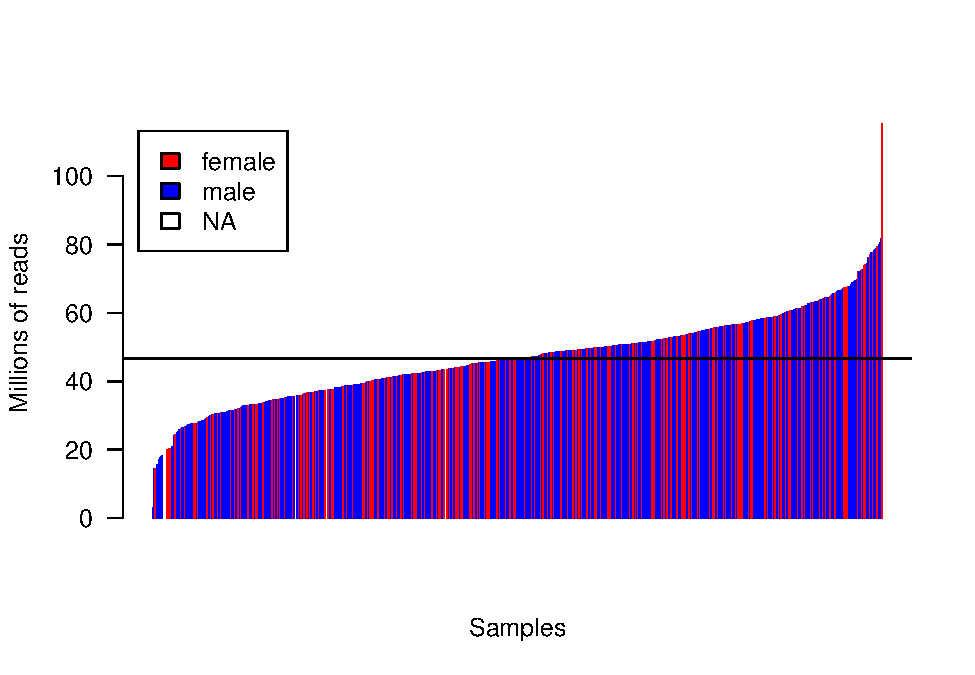
\includegraphics{IEO_project_files/figure-latex/Sequencing depth-1.pdf}

EXPLAIN 21 THRESHOLD AND 614 --\textgreater{} 596

\begin{Shaded}
\begin{Highlighting}[]
\NormalTok{cpm_cutoff <-}\StringTok{ }\DecValTok{21}
\NormalTok{mask <-}\StringTok{ }\KeywordTok{colSums}\NormalTok{(}\KeywordTok{assays}\NormalTok{(se)$counts)/}\FloatTok{1e6} \NormalTok{>}\StringTok{ }\NormalTok{cpm_cutoff}
\NormalTok{se.filt <-}\StringTok{ }\NormalTok{se[, mask]}
\NormalTok{dge.filt <-}\StringTok{ }\NormalTok{dge[, mask]}
\KeywordTok{dim}\NormalTok{(se.filt)}
\end{Highlighting}
\end{Shaded}

\begin{verbatim}
## [1] 20115   596
\end{verbatim}

Store un-normalized versions of the data filtered by sample depth
(cutoff of 21 CPM).

\begin{Shaded}
\begin{Highlighting}[]
\KeywordTok{saveRDS}\NormalTok{(se.filt, }\KeywordTok{file.path}\NormalTok{(}\StringTok{"results"}\NormalTok{, }\StringTok{"se.filt.unnorm.rds"}\NormalTok{))}
\KeywordTok{saveRDS}\NormalTok{(dge.filt, }\KeywordTok{file.path}\NormalTok{(}\StringTok{"results"}\NormalTok{, }\StringTok{"dge.filt.unnorm.rds"}\NormalTok{))}
\end{Highlighting}
\end{Shaded}

\subsubsection{2.4. Distribution of expression levels among
samples}\label{distribution-of-expression-levels-among-samples}

Let's look at the distribution of expression values per sample in terms
of logarithmic CPM units. EXPLAIN PLOTS.

\begin{Shaded}
\begin{Highlighting}[]
\KeywordTok{library}\NormalTok{(geneplotter)}
\end{Highlighting}
\end{Shaded}

\begin{verbatim}
## Warning: package 'geneplotter' was built under R version 3.4.2
\end{verbatim}

\begin{verbatim}
## Loading required package: lattice
\end{verbatim}

\begin{verbatim}
## Loading required package: annotate
\end{verbatim}

\begin{verbatim}
## Warning: package 'annotate' was built under R version 3.4.4
\end{verbatim}

\begin{verbatim}
## Loading required package: AnnotationDbi
\end{verbatim}

\begin{verbatim}
## Warning: package 'AnnotationDbi' was built under R version 3.4.2
\end{verbatim}

\begin{verbatim}
## Loading required package: XML
\end{verbatim}

\begin{verbatim}
## Warning: package 'XML' was built under R version 3.4.4
\end{verbatim}

\begin{Shaded}
\begin{Highlighting}[]
\KeywordTok{par}\NormalTok{(}\DataTypeTok{mfrow=}\KeywordTok{c}\NormalTok{(}\DecValTok{1}\NormalTok{, }\DecValTok{2}\NormalTok{))}
\KeywordTok{multidensity}\NormalTok{(}\KeywordTok{as.list}\NormalTok{(}\KeywordTok{as.data.frame}\NormalTok{(}\KeywordTok{assays}\NormalTok{(se[, se$type ==}\StringTok{ "tumor"}\NormalTok{])$logCPM)),}
             \DataTypeTok{xlab=}\StringTok{"log 2 CPM"}\NormalTok{, }\DataTypeTok{legend=}\OtherTok{NULL}\NormalTok{, }\DataTypeTok{main=}\StringTok{"tumor"}\NormalTok{, }\DataTypeTok{las=}\DecValTok{1}\NormalTok{)}
\KeywordTok{multidensity}\NormalTok{(}\KeywordTok{as.list}\NormalTok{(}\KeywordTok{as.data.frame}\NormalTok{(}\KeywordTok{assays}\NormalTok{(se[, se$type ==}\StringTok{ "normal"}\NormalTok{])$logCPM)),}
             \DataTypeTok{xlab=}\StringTok{"log 2 CPM"}\NormalTok{, }\DataTypeTok{legend=}\OtherTok{NULL}\NormalTok{, }\DataTypeTok{main=}\StringTok{"normal"}\NormalTok{, }\DataTypeTok{las=}\DecValTok{1}\NormalTok{)}
\end{Highlighting}
\end{Shaded}

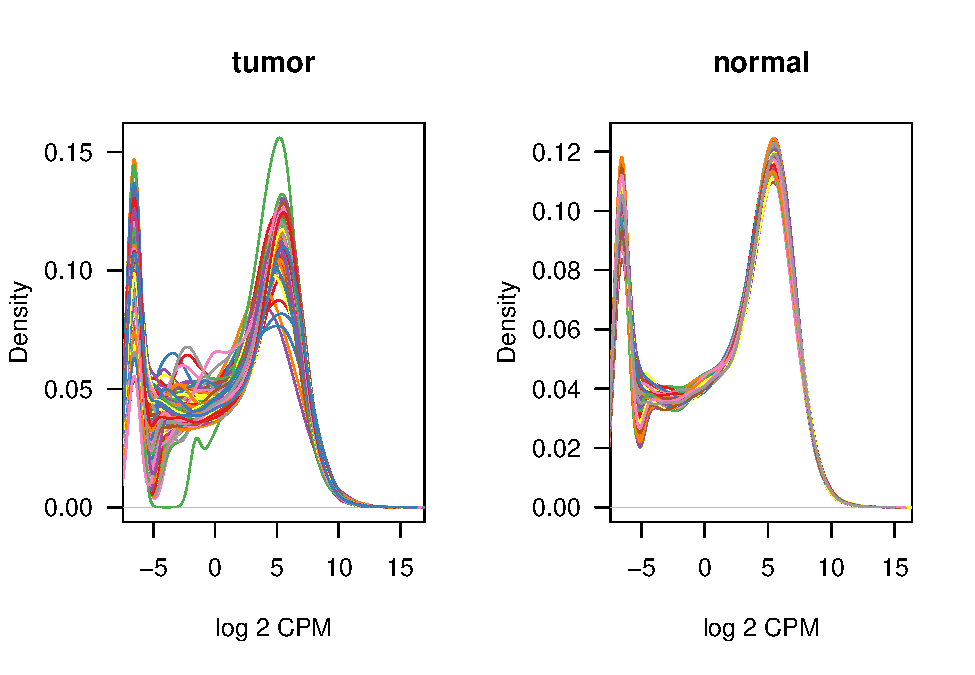
\includegraphics{IEO_project_files/figure-latex/Distribution of expression levels among samples-1.pdf}

\subsubsection{2.5. Distribution and filtering of expression levels
among
genes}\label{distribution-and-filtering-of-expression-levels-among-genes}

Let's calculate now the average expression per gene through all the
samples.

\begin{Shaded}
\begin{Highlighting}[]
\NormalTok{cpm_cutoff <-}\StringTok{ }\KeywordTok{round}\NormalTok{(}\DecValTok{15}\NormalTok{/}\KeywordTok{min}\NormalTok{(dge.filt$samples$lib.size/}\FloatTok{1e+06}\NormalTok{), }\DataTypeTok{digits =} \DecValTok{1}\NormalTok{)}
\NormalTok{cpm_cutoff}
\end{Highlighting}
\end{Shaded}

\begin{verbatim}
## [1] 0.6
\end{verbatim}

\begin{Shaded}
\begin{Highlighting}[]
\NormalTok{nsamplescutoff <-}\StringTok{ }\KeywordTok{min}\NormalTok{(}\KeywordTok{table}\NormalTok{(se.filt$type))}
\NormalTok{nsamplescutoff}
\end{Highlighting}
\end{Shaded}

\begin{verbatim}
## [1] 72
\end{verbatim}

\begin{Shaded}
\begin{Highlighting}[]
\NormalTok{mask <-}\StringTok{ }\KeywordTok{rowSums}\NormalTok{(}\KeywordTok{cpm}\NormalTok{(dge.filt) >}\StringTok{ }\NormalTok{cpm_cutoff) >=}\StringTok{ }\NormalTok{nsamplescutoff}
\NormalTok{se.filt2 <-}\StringTok{ }\NormalTok{se.filt[mask, ]}
\NormalTok{dge.filt2 <-}\StringTok{ }\NormalTok{dge.filt[mask, ]}
\NormalTok{avgexp <-}\StringTok{ }\KeywordTok{rowMeans}\NormalTok{(}\KeywordTok{assays}\NormalTok{(se.filt)$logCPM)}

\KeywordTok{par}\NormalTok{(}\DataTypeTok{mar =} \KeywordTok{c}\NormalTok{(}\DecValTok{4}\NormalTok{, }\DecValTok{5}\NormalTok{, }\DecValTok{1}\NormalTok{, }\DecValTok{1}\NormalTok{))}
\NormalTok{h <-}\StringTok{ }\KeywordTok{hist}\NormalTok{(avgexp, }\DataTypeTok{xlab =} \KeywordTok{expression}\NormalTok{(}\StringTok{"Expression level ("} \NormalTok{*}\StringTok{ }\NormalTok{log[}\DecValTok{2}\NormalTok{] *}\StringTok{ "CPM)"}\NormalTok{), }\DataTypeTok{main =} \StringTok{""}\NormalTok{, }
    \DataTypeTok{las =} \DecValTok{1}\NormalTok{, }\DataTypeTok{col =} \StringTok{"grey"}\NormalTok{, }\DataTypeTok{cex.axis =} \FloatTok{1.2}\NormalTok{, }\DataTypeTok{cex.lab =} \FloatTok{1.5}\NormalTok{)}
\end{Highlighting}
\end{Shaded}

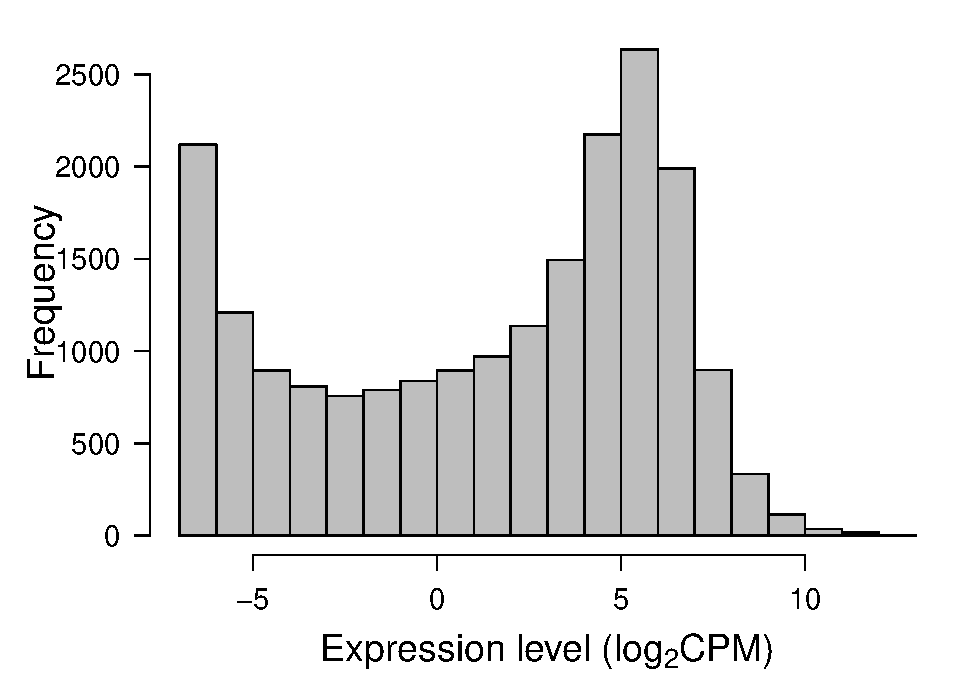
\includegraphics{IEO_project_files/figure-latex/Distribution of expression levels among genes-1.pdf}

EXPLAIN THE DOUBLE CUTOFF.

\begin{Shaded}
\begin{Highlighting}[]
\KeywordTok{par}\NormalTok{(}\DataTypeTok{mar =} \KeywordTok{c}\NormalTok{(}\DecValTok{4}\NormalTok{, }\DecValTok{5}\NormalTok{, }\DecValTok{1}\NormalTok{, }\DecValTok{1}\NormalTok{))}
\NormalTok{h <-}\StringTok{ }\KeywordTok{hist}\NormalTok{(avgexp, }\DataTypeTok{xlab =} \KeywordTok{expression}\NormalTok{(}\StringTok{"Expression level ("} \NormalTok{*}\StringTok{ }\NormalTok{log[}\DecValTok{2}\NormalTok{] *}\StringTok{ "CPM)"}\NormalTok{), }\DataTypeTok{main =} \StringTok{""}\NormalTok{, }
    \DataTypeTok{las =} \DecValTok{1}\NormalTok{, }\DataTypeTok{col =} \StringTok{"grey"}\NormalTok{, }\DataTypeTok{cex.axis =} \FloatTok{1.2}\NormalTok{, }\DataTypeTok{cex.lab =} \FloatTok{1.5}\NormalTok{)}
\NormalTok{x <-}\StringTok{ }\KeywordTok{cut}\NormalTok{(}\KeywordTok{rowMeans}\NormalTok{(}\KeywordTok{assays}\NormalTok{(se.filt2)$logCPM), }\DataTypeTok{breaks =} \NormalTok{h$breaks)}
\KeywordTok{lines}\NormalTok{(h$mids, }\KeywordTok{table}\NormalTok{(x), }\DataTypeTok{type =} \StringTok{"h"}\NormalTok{, }\DataTypeTok{lwd =} \DecValTok{10}\NormalTok{, }\DataTypeTok{lend =} \DecValTok{1}\NormalTok{, }\DataTypeTok{col =} \StringTok{"darkred"}\NormalTok{)}
\KeywordTok{legend}\NormalTok{(}\StringTok{"topleft"}\NormalTok{, }\KeywordTok{c}\NormalTok{(}\StringTok{"All genes"}\NormalTok{, }\StringTok{"Filtered genes"}\NormalTok{), }\DataTypeTok{fill =} \KeywordTok{c}\NormalTok{(}\StringTok{"grey"}\NormalTok{, }\StringTok{"darkred"}\NormalTok{))}
\end{Highlighting}
\end{Shaded}

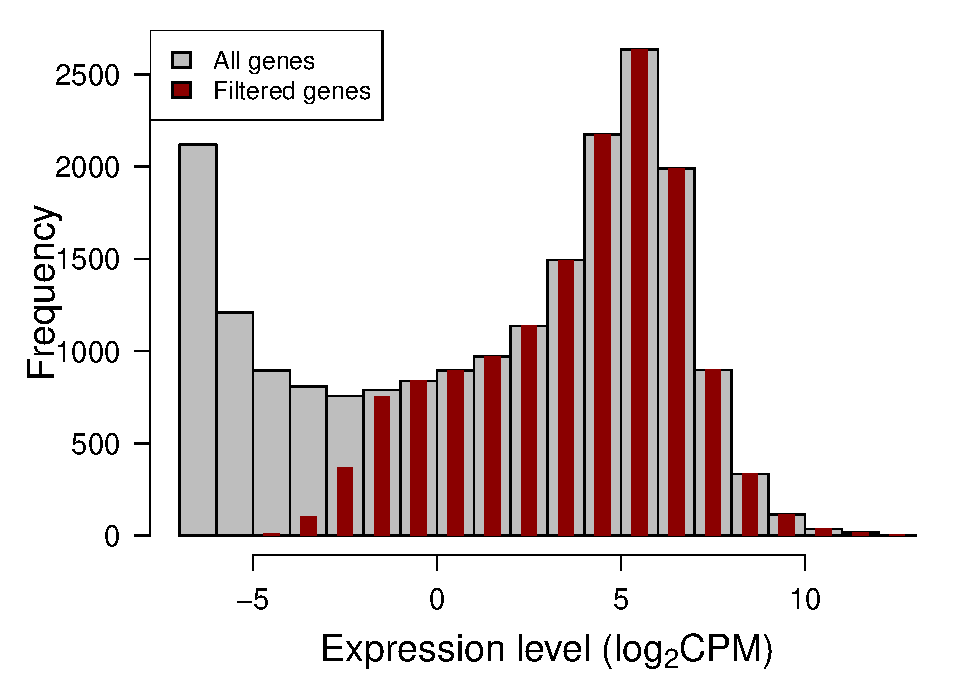
\includegraphics{IEO_project_files/figure-latex/unnamed-chunk-2-1.pdf}

Store un-normalized versions of the data filtered by gene expression
(cutoff of 0.6 CPM expressed in at least 72 samples).

\begin{Shaded}
\begin{Highlighting}[]
\KeywordTok{saveRDS}\NormalTok{(se.filt2, }\KeywordTok{file.path}\NormalTok{(}\StringTok{"results"}\NormalTok{, }\StringTok{"se.filt2.unnorm.rds"}\NormalTok{))}
\KeywordTok{saveRDS}\NormalTok{(dge.filt2, }\KeywordTok{file.path}\NormalTok{(}\StringTok{"results"}\NormalTok{, }\StringTok{"dge.filt2.unnorm.rds"}\NormalTok{))}
\end{Highlighting}
\end{Shaded}

\subsubsection{2.6. Between-sample
normalization}\label{between-sample-normalization}

We calculate now the normalization factors on the filtered expression
data set.

\begin{Shaded}
\begin{Highlighting}[]
\NormalTok{dge.filt2 <-}\StringTok{ }\KeywordTok{calcNormFactors}\NormalTok{(dge.filt2)}
\NormalTok{dge.filt$samples$group <-}\StringTok{ }\NormalTok{se.filt$type}
\NormalTok{dge.filt2$samples$group <-}\StringTok{ }\NormalTok{se.filt2$type}
\KeywordTok{table}\NormalTok{(dge.filt2$samples$group)}
\end{Highlighting}
\end{Shaded}

\begin{verbatim}
## 
## normal  tumor 
##     72    524
\end{verbatim}

\begin{Shaded}
\begin{Highlighting}[]
\KeywordTok{par}\NormalTok{(}\DataTypeTok{mfrow =} \KeywordTok{c}\NormalTok{(}\DecValTok{1}\NormalTok{, }\DecValTok{2}\NormalTok{))}
\KeywordTok{plotSmear}\NormalTok{(dge.filt, }\DataTypeTok{lowess =} \OtherTok{TRUE}\NormalTok{, }\DataTypeTok{las =} \DecValTok{1}\NormalTok{, }\DataTypeTok{cex.lab =} \FloatTok{1.5}\NormalTok{, }\DataTypeTok{cex.axis =} \FloatTok{1.2}\NormalTok{)}
\KeywordTok{abline}\NormalTok{(}\DataTypeTok{h =} \DecValTok{0}\NormalTok{, }\DataTypeTok{col =} \StringTok{"blue"}\NormalTok{, }\DataTypeTok{lwd =} \DecValTok{2}\NormalTok{)}
\KeywordTok{plotSmear}\NormalTok{(dge.filt2, }\DataTypeTok{lowess =} \OtherTok{TRUE}\NormalTok{, }\DataTypeTok{las =} \DecValTok{1}\NormalTok{, }\DataTypeTok{cex.lab =} \FloatTok{1.5}\NormalTok{, }\DataTypeTok{cex.axis =} \FloatTok{1.2}\NormalTok{)}
\KeywordTok{abline}\NormalTok{(}\DataTypeTok{h =} \DecValTok{0}\NormalTok{, }\DataTypeTok{col =} \StringTok{"blue"}\NormalTok{, }\DataTypeTok{lwd =} \DecValTok{2}\NormalTok{)}
\end{Highlighting}
\end{Shaded}

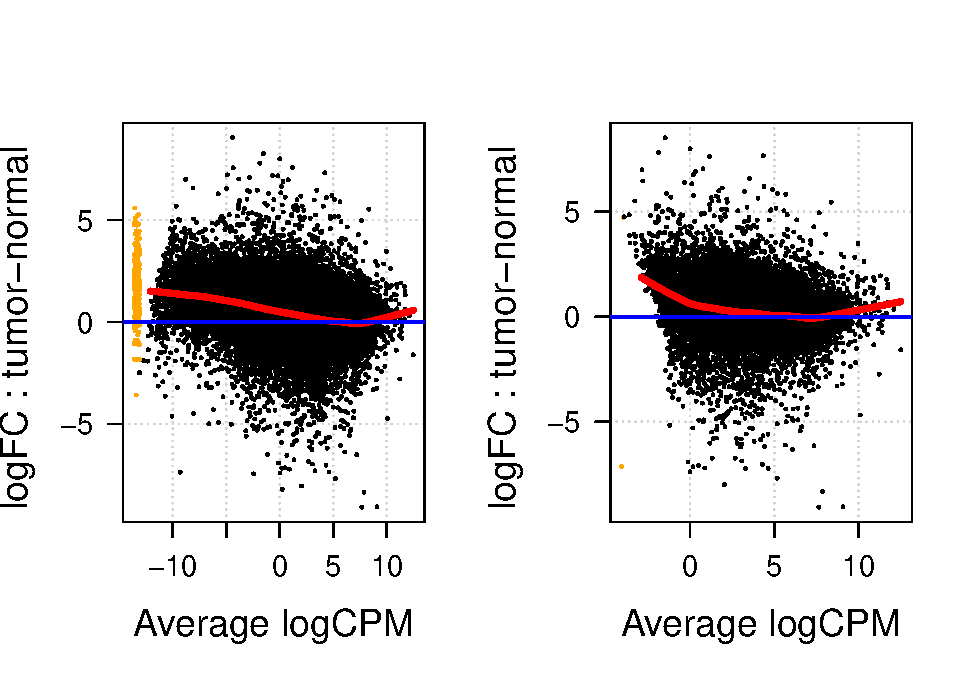
\includegraphics{IEO_project_files/figure-latex/Between-sample normalization-1.pdf}

\subsubsection{2.7. Batch Identification}\label{batch-identification}

EXPLANATION BATCHES and BATCH filtering

\begin{Shaded}
\begin{Highlighting}[]
\NormalTok{tss <-}\StringTok{ }\KeywordTok{substr}\NormalTok{(}\KeywordTok{colnames}\NormalTok{(se.filt2), }\DecValTok{6}\NormalTok{, }\DecValTok{7}\NormalTok{)}
\NormalTok{center <-}\StringTok{ }\KeywordTok{substr}\NormalTok{(}\KeywordTok{colnames}\NormalTok{(se.filt2), }\DecValTok{27}\NormalTok{, }\DecValTok{28}\NormalTok{)}
\NormalTok{plate <-}\StringTok{ }\KeywordTok{substr}\NormalTok{(}\KeywordTok{colnames}\NormalTok{(se.filt2), }\DecValTok{22}\NormalTok{, }\DecValTok{25}\NormalTok{)}
\NormalTok{portionanalyte <-}\StringTok{ }\KeywordTok{substr}\NormalTok{(}\KeywordTok{colnames}\NormalTok{(se.filt2), }\DecValTok{18}\NormalTok{, }\DecValTok{20}\NormalTok{)}
\NormalTok{samplevial <-}\StringTok{ }\KeywordTok{substr}\NormalTok{(}\KeywordTok{colnames}\NormalTok{(se.filt2), }\DecValTok{14}\NormalTok{, }\DecValTok{16}\NormalTok{)}

\KeywordTok{table}\NormalTok{(}\KeywordTok{data.frame}\NormalTok{(}\DataTypeTok{TYPE=}\NormalTok{se.filt2$type, }\DataTypeTok{TSS=}\NormalTok{tss))}
\end{Highlighting}
\end{Shaded}

\begin{verbatim}
##         TSS
## TYPE      3Z  6D  A3  AK  AS  B0  B2  B4  B8  BP  CJ  CW  CZ  DV  EU  G6
##   normal   0   0   2   0   0  16   2   0   5   0  10  10  27   0   0   0
##   tumor    1   1  50  22   2 103  15   9  31 140  69  15  40  13   4   3
##         TSS
## TYPE      GK  MM  MW  T7
##   normal   0   0   0   0
##   tumor    1   3   1   1
\end{verbatim}

\begin{Shaded}
\begin{Highlighting}[]
\KeywordTok{table}\NormalTok{(}\KeywordTok{data.frame}\NormalTok{(}\DataTypeTok{TYPE=}\NormalTok{se.filt2$type, }\DataTypeTok{PLATE=}\NormalTok{plate))}
\end{Highlighting}
\end{Shaded}

\begin{verbatim}
##         PLATE
## TYPE     0864 1188 1277 1289 1305 1325 1334 1420 1426 1503 1541 1672 1758
##   normal    0    0    0    0    0    0    0    0    0   22   31   15    3
##   tumor    16    6   39   49   46   46   47   47   45   44   59   41    0
##         PLATE
## TYPE     1766 1858 A266 A277 A32Z A33J A37O A39I
##   normal    0    1    0    0    0    0    0    0
##   tumor     2    0   10    3    1   10   12    1
\end{verbatim}

\begin{Shaded}
\begin{Highlighting}[]
\KeywordTok{table}\NormalTok{(}\KeywordTok{data.frame}\NormalTok{(}\DataTypeTok{TYPE=}\NormalTok{se.filt2$type, }\DataTypeTok{SAMPLEVIAL=}\NormalTok{samplevial))}
\end{Highlighting}
\end{Shaded}

\begin{verbatim}
##         SAMPLEVIAL
## TYPE     01A 01B 05A 11A
##   normal   0   0   0  72
##   tumor  520   3   1   0
\end{verbatim}

\begin{Shaded}
\begin{Highlighting}[]
\KeywordTok{table}\NormalTok{(}\KeywordTok{data.frame}\NormalTok{(}\DataTypeTok{TYPE=}\NormalTok{se.filt2$type, }\DataTypeTok{PORTIONANALYTE=}\NormalTok{portionanalyte))}
\end{Highlighting}
\end{Shaded}

\begin{verbatim}
##         PORTIONANALYTE
## TYPE     01R 02R 03R 11R 12R 13R 21R
##   normal  69   3   0   0   0   0   0
##   tumor  308 115   1  94   3   1   2
\end{verbatim}

\begin{Shaded}
\begin{Highlighting}[]
\NormalTok{tss_list <-}\StringTok{ }\KeywordTok{c}\NormalTok{(}\StringTok{"A3"}\NormalTok{,}\StringTok{"B0"}\NormalTok{,}\StringTok{"B2"}\NormalTok{,}\StringTok{"B8"}\NormalTok{,}\StringTok{"CW"}\NormalTok{,}\StringTok{"CZ"}\NormalTok{)}
\NormalTok{plate_list <-}\StringTok{ }\KeywordTok{c}\NormalTok{(}\DecValTok{1503}\NormalTok{,}\DecValTok{1541}\NormalTok{,}\DecValTok{1672}\NormalTok{)}
\NormalTok{samplevial_list <-}\StringTok{ }\KeywordTok{c}\NormalTok{(}\StringTok{"01A"}\NormalTok{,}\StringTok{"11A"}\NormalTok{)}
\NormalTok{portion <-}\StringTok{ "01R"}
\NormalTok{the_mask <-}\StringTok{ }\NormalTok{(}\KeywordTok{substr}\NormalTok{(}\KeywordTok{colnames}\NormalTok{(dge.filt),}\DecValTok{6}\NormalTok{,}\DecValTok{7}\NormalTok{) %in%}\StringTok{ }\NormalTok{tss_list &}\StringTok{ }\KeywordTok{substr}\NormalTok{(}\KeywordTok{colnames}\NormalTok{(dge.filt),}\DecValTok{22}\NormalTok{,}\DecValTok{25}\NormalTok{) %in%}\StringTok{ }\NormalTok{plate_list &}\StringTok{ }\KeywordTok{substr}\NormalTok{(}\KeywordTok{colnames}\NormalTok{(dge.filt),}\DecValTok{18}\NormalTok{,}\DecValTok{20}\NormalTok{) ==}\StringTok{ }\NormalTok{portion &}\StringTok{ }\KeywordTok{substr}\NormalTok{(}\KeywordTok{colnames}\NormalTok{(dge.filt),}\DecValTok{14}\NormalTok{,}\DecValTok{16}\NormalTok{) %in%}\StringTok{ }\NormalTok{samplevial_list)}

\NormalTok{se.filt3 <-}\StringTok{ }\NormalTok{se.filt2[,the_mask]}
\NormalTok{dge.filt3 <-}\StringTok{ }\NormalTok{dge.filt2[,the_mask]}

\NormalTok{tss2 <-}\StringTok{ }\KeywordTok{substr}\NormalTok{(}\KeywordTok{colnames}\NormalTok{(se.filt3), }\DecValTok{6}\NormalTok{, }\DecValTok{7}\NormalTok{)}
\NormalTok{plate2 <-}\StringTok{ }\KeywordTok{substr}\NormalTok{(}\KeywordTok{colnames}\NormalTok{(se.filt3), }\DecValTok{22}\NormalTok{, }\DecValTok{25}\NormalTok{)}
\NormalTok{portionanalyte2 <-}\StringTok{ }\KeywordTok{substr}\NormalTok{(}\KeywordTok{colnames}\NormalTok{(se.filt3), }\DecValTok{18}\NormalTok{, }\DecValTok{20}\NormalTok{)}
\NormalTok{samplevial2 <-}\StringTok{ }\KeywordTok{substr}\NormalTok{(}\KeywordTok{colnames}\NormalTok{(se.filt3), }\DecValTok{14}\NormalTok{, }\DecValTok{16}\NormalTok{)}

\KeywordTok{table}\NormalTok{(}\KeywordTok{data.frame}\NormalTok{(}\DataTypeTok{TYPE=}\NormalTok{se.filt3$type, }\DataTypeTok{TSS=}\NormalTok{tss2))}
\end{Highlighting}
\end{Shaded}

\begin{verbatim}
##         TSS
## TYPE     A3 B0 B2 B8 CW CZ
##   normal  2 15  2  2  9 26
##   tumor   2 15  4  7  8 23
\end{verbatim}

\begin{Shaded}
\begin{Highlighting}[]
\KeywordTok{table}\NormalTok{(}\KeywordTok{data.frame}\NormalTok{(}\DataTypeTok{TYPE=}\NormalTok{se.filt3$type, }\DataTypeTok{PLATE=}\NormalTok{plate2))}
\end{Highlighting}
\end{Shaded}

\begin{verbatim}
##         PLATE
## TYPE     1503 1541 1672
##   normal   20   23   13
##   tumor    39   18    2
\end{verbatim}

\begin{Shaded}
\begin{Highlighting}[]
\KeywordTok{table}\NormalTok{(}\KeywordTok{data.frame}\NormalTok{(}\DataTypeTok{TYPE=}\NormalTok{se.filt3$type, }\DataTypeTok{SAMPLEVIAL=}\NormalTok{samplevial2))}
\end{Highlighting}
\end{Shaded}

\begin{verbatim}
##         SAMPLEVIAL
## TYPE     01A 11A
##   normal   0  56
##   tumor   59   0
\end{verbatim}

\begin{Shaded}
\begin{Highlighting}[]
\KeywordTok{table}\NormalTok{(}\KeywordTok{data.frame}\NormalTok{(}\DataTypeTok{TYPE=}\NormalTok{se.filt3$type, }\DataTypeTok{PORTIONANALYTE=}\NormalTok{portionanalyte2))}
\end{Highlighting}
\end{Shaded}

\begin{verbatim}
##         PORTIONANALYTE
## TYPE     01R
##   normal  56
##   tumor   59
\end{verbatim}

\subsubsection{2.8. Clustering according to batch
effect}\label{clustering-according-to-batch-effect}

\begin{Shaded}
\begin{Highlighting}[]
\NormalTok{logCPM <-}\StringTok{ }\KeywordTok{cpm}\NormalTok{(dge.filt3, }\DataTypeTok{log=}\OtherTok{TRUE}\NormalTok{, }\DataTypeTok{prior.count=}\DecValTok{3}\NormalTok{)}
\NormalTok{d <-}\StringTok{ }\KeywordTok{as.dist}\NormalTok{(}\DecValTok{1}\NormalTok{-}\KeywordTok{cor}\NormalTok{(logCPM, }\DataTypeTok{method=}\StringTok{"spearman"}\NormalTok{))}
\NormalTok{sampleClustering <-}\StringTok{ }\KeywordTok{hclust}\NormalTok{(d)}
\NormalTok{batch <-}\StringTok{ }\KeywordTok{as.integer}\NormalTok{(}\KeywordTok{factor}\NormalTok{(tss2))}
\NormalTok{sampleDendrogram <-}\StringTok{ }\KeywordTok{as.dendrogram}\NormalTok{(sampleClustering, }\DataTypeTok{hang=}\FloatTok{0.1}\NormalTok{)}
\KeywordTok{names}\NormalTok{(batch) <-}\StringTok{ }\KeywordTok{colnames}\NormalTok{(se.filt3)}
\NormalTok{outcome <-}\StringTok{ }\KeywordTok{paste}\NormalTok{(}\KeywordTok{substr}\NormalTok{(}\KeywordTok{colnames}\NormalTok{(se.filt3), }\DecValTok{9}\NormalTok{, }\DecValTok{12}\NormalTok{), }\KeywordTok{as.character}\NormalTok{(se.filt3$type), }\DataTypeTok{sep=}\StringTok{"-"}\NormalTok{)}
\KeywordTok{names}\NormalTok{(outcome) <-}\StringTok{ }\KeywordTok{colnames}\NormalTok{(se.filt3)}
\NormalTok{sampleDendrogram <-}\StringTok{ }\KeywordTok{dendrapply}\NormalTok{(sampleDendrogram,}
                               \NormalTok{function(x, batch, labels) \{}
                                 \NormalTok{if (}\KeywordTok{is.leaf}\NormalTok{(x)) \{}
                                   \KeywordTok{attr}\NormalTok{(x, }\StringTok{"nodePar"}\NormalTok{) <-}\StringTok{ }\KeywordTok{list}\NormalTok{(}\DataTypeTok{lab.col=}\KeywordTok{as.vector}\NormalTok{(batch[}\KeywordTok{attr}\NormalTok{(x, }\StringTok{"label"}\NormalTok{)]))}
                                   \KeywordTok{attr}\NormalTok{(x, }\StringTok{"label"}\NormalTok{) <-}\StringTok{ }\KeywordTok{as.vector}\NormalTok{(labels[}\KeywordTok{attr}\NormalTok{(x, }\StringTok{"label"}\NormalTok{)])}
                                 \NormalTok{\}}
                                 \NormalTok{x}
                               \NormalTok{\}, batch, outcome)}
\KeywordTok{plot}\NormalTok{(sampleDendrogram, }\DataTypeTok{main=}\StringTok{"Hierarchical clustering of samples"}\NormalTok{)}
\KeywordTok{legend}\NormalTok{(}\StringTok{"topright"}\NormalTok{, }\KeywordTok{paste}\NormalTok{(}\StringTok{"Batch"}\NormalTok{, }\KeywordTok{sort}\NormalTok{(}\KeywordTok{unique}\NormalTok{(batch)), }\KeywordTok{levels}\NormalTok{(}\KeywordTok{factor}\NormalTok{(tss2))), }\DataTypeTok{fill=}\KeywordTok{sort}\NormalTok{(}\KeywordTok{unique}\NormalTok{(batch)))}
\end{Highlighting}
\end{Shaded}

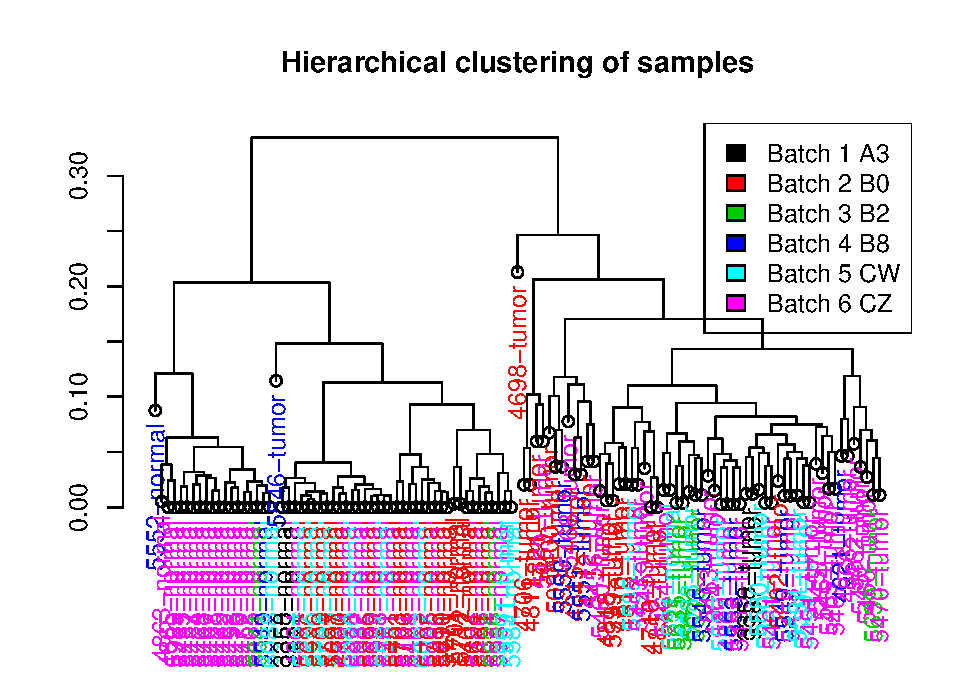
\includegraphics{IEO_project_files/figure-latex/Hierarchical clustering according to batch effect-1.pdf}

\begin{Shaded}
\begin{Highlighting}[]
\NormalTok{batch <-}\StringTok{ }\KeywordTok{as.integer}\NormalTok{(}\KeywordTok{factor}\NormalTok{(plate2))}
\NormalTok{sampleDendrogram <-}\StringTok{ }\KeywordTok{as.dendrogram}\NormalTok{(sampleClustering, }\DataTypeTok{hang=}\FloatTok{0.1}\NormalTok{)}
\KeywordTok{names}\NormalTok{(batch) <-}\StringTok{ }\KeywordTok{colnames}\NormalTok{(se.filt3)}
\NormalTok{outcome <-}\StringTok{ }\KeywordTok{paste}\NormalTok{(}\KeywordTok{substr}\NormalTok{(}\KeywordTok{colnames}\NormalTok{(se.filt3), }\DecValTok{9}\NormalTok{, }\DecValTok{12}\NormalTok{), }\KeywordTok{as.character}\NormalTok{(se.filt3$type), }\DataTypeTok{sep=}\StringTok{"-"}\NormalTok{)}
\KeywordTok{names}\NormalTok{(outcome) <-}\StringTok{ }\KeywordTok{colnames}\NormalTok{(se.filt3)}
\NormalTok{sampleDendrogram <-}\StringTok{ }\KeywordTok{dendrapply}\NormalTok{(sampleDendrogram,}
                               \NormalTok{function(x, batch, labels) \{}
                                 \NormalTok{if (}\KeywordTok{is.leaf}\NormalTok{(x)) \{}
                                   \KeywordTok{attr}\NormalTok{(x, }\StringTok{"nodePar"}\NormalTok{) <-}\StringTok{ }\KeywordTok{list}\NormalTok{(}\DataTypeTok{lab.col=}\KeywordTok{as.vector}\NormalTok{(batch[}\KeywordTok{attr}\NormalTok{(x, }\StringTok{"label"}\NormalTok{)]))}
                                   \KeywordTok{attr}\NormalTok{(x, }\StringTok{"label"}\NormalTok{) <-}\StringTok{ }\KeywordTok{as.vector}\NormalTok{(labels[}\KeywordTok{attr}\NormalTok{(x, }\StringTok{"label"}\NormalTok{)])}
                                 \NormalTok{\}}
                                 \NormalTok{x}
                               \NormalTok{\}, batch, outcome)}
\KeywordTok{plot}\NormalTok{(sampleDendrogram, }\DataTypeTok{main=}\StringTok{"Hierarchical clustering of samples"}\NormalTok{)}
\KeywordTok{legend}\NormalTok{(}\StringTok{"topright"}\NormalTok{, }\KeywordTok{paste}\NormalTok{(}\StringTok{"Batch"}\NormalTok{, }\KeywordTok{sort}\NormalTok{(}\KeywordTok{unique}\NormalTok{(batch)), }\KeywordTok{levels}\NormalTok{(}\KeywordTok{factor}\NormalTok{(plate2))), }\DataTypeTok{fill=}\KeywordTok{sort}\NormalTok{(}\KeywordTok{unique}\NormalTok{(batch)))}
\end{Highlighting}
\end{Shaded}

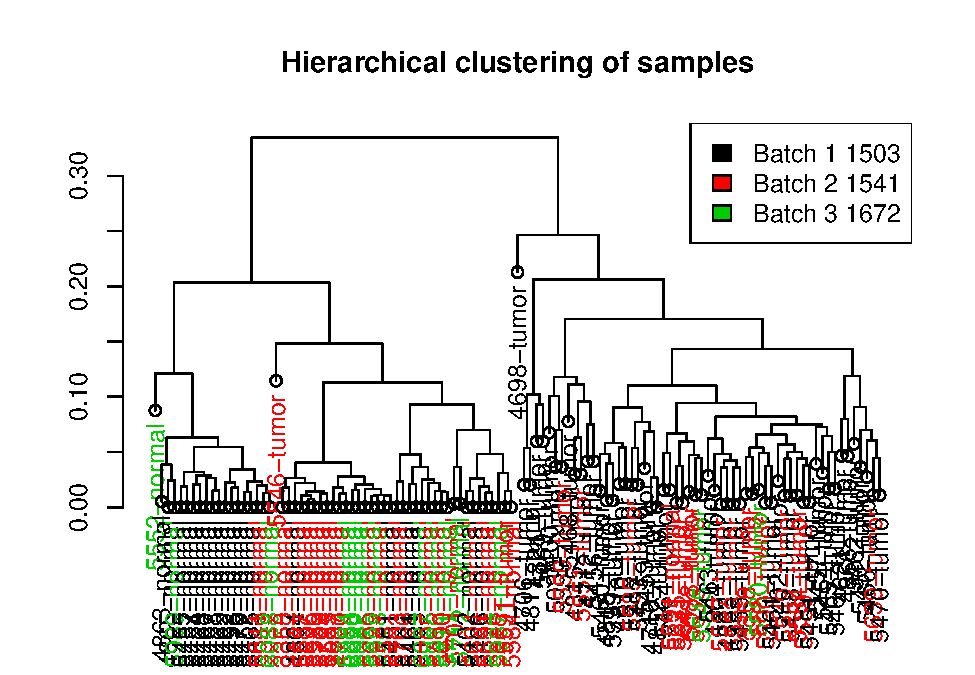
\includegraphics{IEO_project_files/figure-latex/Hierarchical clustering according to batch effect-2.pdf}

\begin{Shaded}
\begin{Highlighting}[]
\NormalTok{batch <-}\StringTok{ }\KeywordTok{as.integer}\NormalTok{(}\KeywordTok{factor}\NormalTok{(samplevial2))}
\NormalTok{sampleDendrogram <-}\StringTok{ }\KeywordTok{as.dendrogram}\NormalTok{(sampleClustering, }\DataTypeTok{hang=}\FloatTok{0.1}\NormalTok{)}
\KeywordTok{names}\NormalTok{(batch) <-}\StringTok{ }\KeywordTok{colnames}\NormalTok{(se.filt3)}
\NormalTok{outcome <-}\StringTok{ }\KeywordTok{paste}\NormalTok{(}\KeywordTok{substr}\NormalTok{(}\KeywordTok{colnames}\NormalTok{(se.filt3), }\DecValTok{9}\NormalTok{, }\DecValTok{12}\NormalTok{), }\KeywordTok{as.character}\NormalTok{(se.filt3$type), }\DataTypeTok{sep=}\StringTok{"-"}\NormalTok{)}
\KeywordTok{names}\NormalTok{(outcome) <-}\StringTok{ }\KeywordTok{colnames}\NormalTok{(se.filt3)}
\NormalTok{sampleDendrogram <-}\StringTok{ }\KeywordTok{dendrapply}\NormalTok{(sampleDendrogram,}
                               \NormalTok{function(x, batch, labels) \{}
                                 \NormalTok{if (}\KeywordTok{is.leaf}\NormalTok{(x)) \{}
                                   \KeywordTok{attr}\NormalTok{(x, }\StringTok{"nodePar"}\NormalTok{) <-}\StringTok{ }\KeywordTok{list}\NormalTok{(}\DataTypeTok{lab.col=}\KeywordTok{as.vector}\NormalTok{(batch[}\KeywordTok{attr}\NormalTok{(x, }\StringTok{"label"}\NormalTok{)]))}
                                   \KeywordTok{attr}\NormalTok{(x, }\StringTok{"label"}\NormalTok{) <-}\StringTok{ }\KeywordTok{as.vector}\NormalTok{(labels[}\KeywordTok{attr}\NormalTok{(x, }\StringTok{"label"}\NormalTok{)])}
                                 \NormalTok{\}}
                                 \NormalTok{x}
                               \NormalTok{\}, batch, outcome)}
\KeywordTok{plot}\NormalTok{(sampleDendrogram, }\DataTypeTok{main=}\StringTok{"Hierarchical clustering of samples"}\NormalTok{)}
\KeywordTok{legend}\NormalTok{(}\StringTok{"topright"}\NormalTok{, }\KeywordTok{paste}\NormalTok{(}\StringTok{"Batch"}\NormalTok{, }\KeywordTok{sort}\NormalTok{(}\KeywordTok{unique}\NormalTok{(batch)), }\KeywordTok{levels}\NormalTok{(}\KeywordTok{factor}\NormalTok{(samplevial2))), }\DataTypeTok{fill=}\KeywordTok{sort}\NormalTok{(}\KeywordTok{unique}\NormalTok{(batch)))}
\end{Highlighting}
\end{Shaded}

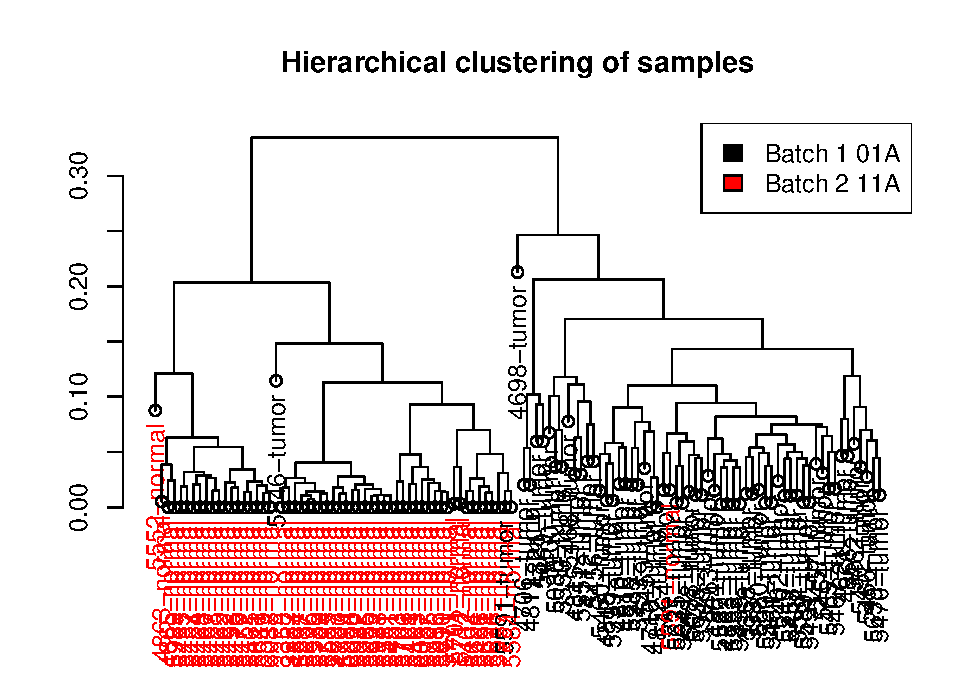
\includegraphics{IEO_project_files/figure-latex/Hierarchical clustering according to batch effect-3.pdf}

\begin{Shaded}
\begin{Highlighting}[]
\NormalTok{se.filt4 <-}\StringTok{ }\NormalTok{se.filt3[,}\KeywordTok{grep}\NormalTok{(}\StringTok{"5546|5591"}\NormalTok{, }\KeywordTok{colnames}\NormalTok{(se.filt3), }\DataTypeTok{invert=}\OtherTok{TRUE}\NormalTok{)]}
\NormalTok{dge.filt4 <-}\StringTok{ }\NormalTok{dge.filt3[,}\KeywordTok{grep}\NormalTok{(}\StringTok{"5546|5591"}\NormalTok{, }\KeywordTok{colnames}\NormalTok{(dge.filt3), }\DataTypeTok{invert=}\OtherTok{TRUE}\NormalTok{)]}
\NormalTok{se.dis <-}\StringTok{ }\NormalTok{se.filt3[,}\KeywordTok{grep}\NormalTok{(}\StringTok{"5546|5591"}\NormalTok{, }\KeywordTok{colnames}\NormalTok{(se.filt3))]}
\NormalTok{tss3 <-}\StringTok{ }\KeywordTok{substr}\NormalTok{(}\KeywordTok{colnames}\NormalTok{(se.filt4), }\DecValTok{6}\NormalTok{, }\DecValTok{7}\NormalTok{)}
\NormalTok{plate3 <-}\StringTok{ }\KeywordTok{substr}\NormalTok{(}\KeywordTok{colnames}\NormalTok{(se.filt4), }\DecValTok{22}\NormalTok{, }\DecValTok{25}\NormalTok{)}
\NormalTok{portionanalyte3 <-}\StringTok{ }\KeywordTok{substr}\NormalTok{(}\KeywordTok{colnames}\NormalTok{(se.filt4), }\DecValTok{18}\NormalTok{, }\DecValTok{20}\NormalTok{)}
\NormalTok{samplevial3 <-}\StringTok{ }\KeywordTok{substr}\NormalTok{(}\KeywordTok{colnames}\NormalTok{(se.filt4), }\DecValTok{14}\NormalTok{, }\DecValTok{16}\NormalTok{)}
\end{Highlighting}
\end{Shaded}

\subsubsection{2.8. Clustering according to batch
effect}\label{clustering-according-to-batch-effect-1}

\begin{Shaded}
\begin{Highlighting}[]
\KeywordTok{colnames}\NormalTok{(dge.filt4) <-}\StringTok{ }\KeywordTok{c}\NormalTok{(}\DecValTok{1}\NormalTok{:}\DecValTok{112}\NormalTok{)}
\KeywordTok{colnames}\NormalTok{(se.filt4) <-}\StringTok{ }\KeywordTok{c}\NormalTok{(}\DecValTok{1}\NormalTok{:}\DecValTok{112}\NormalTok{)}
\NormalTok{tumor_se <-}\StringTok{ }\NormalTok{se.filt4[,se.filt4$type ==}\StringTok{ "tumor"}\NormalTok{]}
\NormalTok{tumor_dge <-}\StringTok{ }\NormalTok{dge.filt4[,se.filt4$type ==}\StringTok{ "tumor"}\NormalTok{]}

\NormalTok{###GENDER}
\NormalTok{se_gender <-}\StringTok{ }\NormalTok{se.filt4[,!}\KeywordTok{is.na}\NormalTok{(se.filt4$gender)]}
\NormalTok{dge_gender <-}\StringTok{ }\NormalTok{dge.filt4[,!}\KeywordTok{is.na}\NormalTok{(se.filt4$gender)]}
\NormalTok{batch <-}\StringTok{ }\KeywordTok{as.integer}\NormalTok{(}\KeywordTok{factor}\NormalTok{(se_gender$gender))}
\NormalTok{outcome <-}\StringTok{ }\KeywordTok{paste}\NormalTok{(}\KeywordTok{factor}\NormalTok{(se_gender$gender), }\KeywordTok{as.character}\NormalTok{(se_gender$type), }\DataTypeTok{sep=}\StringTok{"-"}\NormalTok{)}
\KeywordTok{plotMDS}\NormalTok{(dge_gender, }\DataTypeTok{col =} \NormalTok{batch,}\DataTypeTok{labels =} \NormalTok{outcome, }\DataTypeTok{cex =} \FloatTok{0.7}\NormalTok{)}
\KeywordTok{legend}\NormalTok{(}\StringTok{"topleft"}\NormalTok{, }\KeywordTok{paste}\NormalTok{(}\StringTok{"Batch"}\NormalTok{, }\KeywordTok{sort}\NormalTok{(}\KeywordTok{unique}\NormalTok{(batch)), }\KeywordTok{levels}\NormalTok{(}\KeywordTok{factor}\NormalTok{(se_gender$gender))), }\DataTypeTok{fill=}\KeywordTok{sort}\NormalTok{(}\KeywordTok{unique}\NormalTok{(batch)), }\DataTypeTok{inset=}\FloatTok{0.005}\NormalTok{)}
\end{Highlighting}
\end{Shaded}

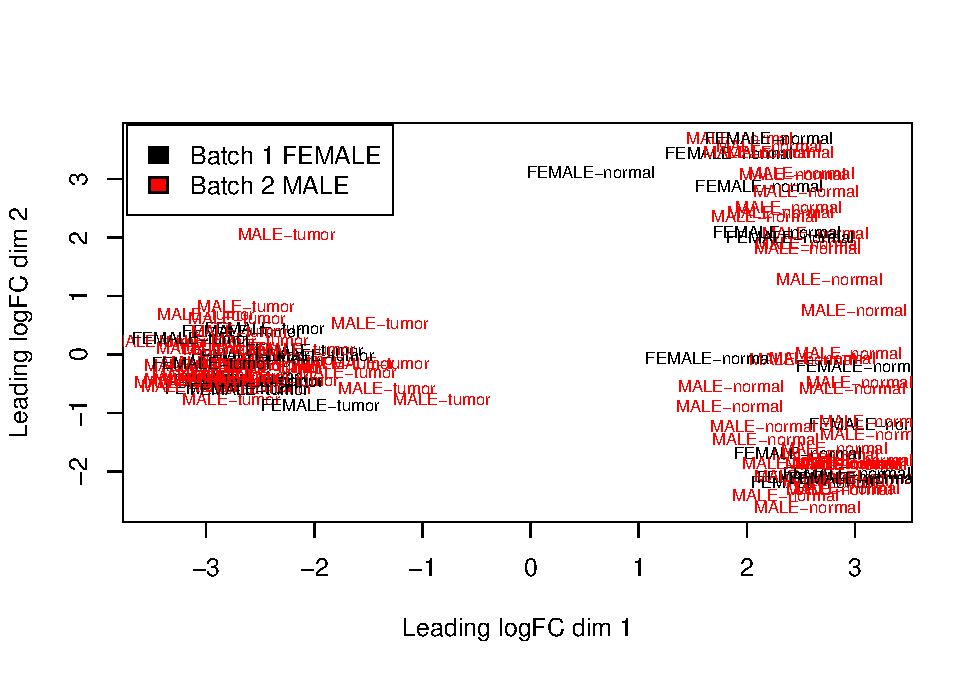
\includegraphics{IEO_project_files/figure-latex/unnamed-chunk-4-1.pdf}

\begin{Shaded}
\begin{Highlighting}[]
\NormalTok{###CANCER STAGE}
\NormalTok{tumor_stage_se <-}\StringTok{ }\NormalTok{tumor_se[,!}\KeywordTok{is.na}\NormalTok{(tumor_se$ajcc_pathologic_tumor_stage)]}
\NormalTok{tumor_stage_dge <-tumor_dge[,!}\KeywordTok{is.na}\NormalTok{(tumor_se$ajcc_pathologic_tumor_stage)]}
\NormalTok{batch <-}\StringTok{ }\KeywordTok{as.integer}\NormalTok{(}\KeywordTok{factor}\NormalTok{(tumor_stage_se$ajcc_pathologic_tumor_stage))}
\NormalTok{outcome <-}\StringTok{ }\KeywordTok{paste}\NormalTok{(}\KeywordTok{factor}\NormalTok{(tumor_stage_se$ajcc_pathologic_tumor_stage), }\KeywordTok{colnames}\NormalTok{(tumor_stage_se), }\DataTypeTok{sep=}\StringTok{"-"}\NormalTok{)}
\KeywordTok{plotMDS}\NormalTok{(tumor_stage_dge, }\DataTypeTok{col =} \NormalTok{batch,}\DataTypeTok{labels =} \NormalTok{outcome, }\DataTypeTok{cex =} \FloatTok{0.7}\NormalTok{)}
\KeywordTok{legend}\NormalTok{(}\StringTok{"bottomright"}\NormalTok{, }\KeywordTok{sort}\NormalTok{(}\KeywordTok{unique}\NormalTok{(batch)), }\KeywordTok{levels}\NormalTok{(}\KeywordTok{factor}\NormalTok{(tumor_stage_se$ajcc_pathologic_tumor_stage)), }\DataTypeTok{fill=}\KeywordTok{sort}\NormalTok{(}\KeywordTok{unique}\NormalTok{(batch)), }\DataTypeTok{inset=}\FloatTok{0.005}\NormalTok{)}
\end{Highlighting}
\end{Shaded}

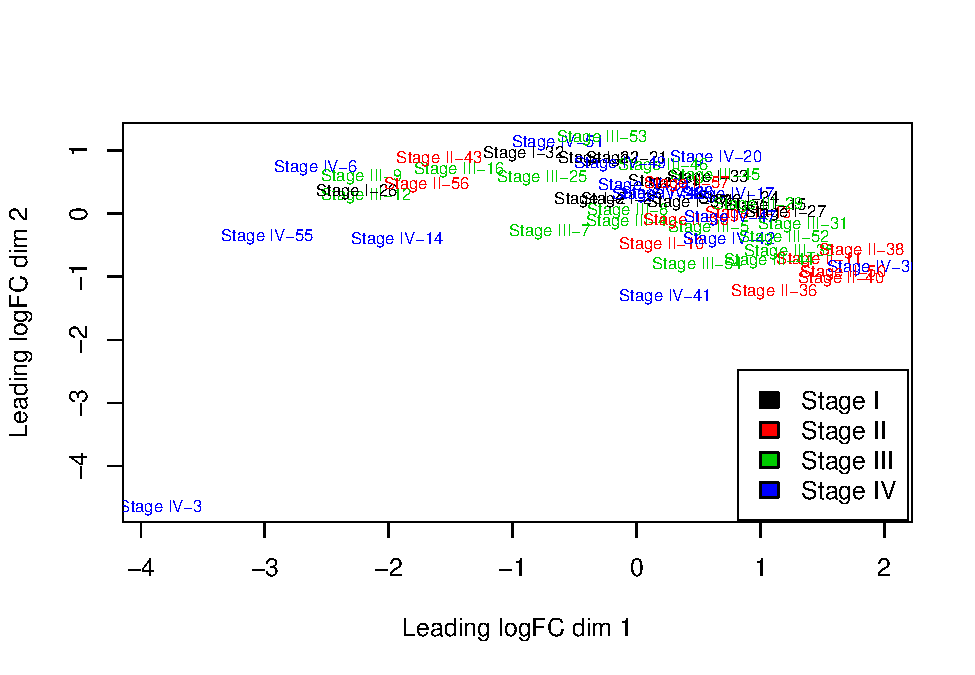
\includegraphics{IEO_project_files/figure-latex/unnamed-chunk-4-2.pdf}

\begin{Shaded}
\begin{Highlighting}[]
\NormalTok{###TUMOR GRADE }
\NormalTok{tumor_grade_se <-}\StringTok{ }\NormalTok{tumor_se[,!}\KeywordTok{is.na}\NormalTok{(tumor_se$tumor_grade)]}
\NormalTok{tumor_grade_dge <-tumor_dge[,!}\KeywordTok{is.na}\NormalTok{(tumor_se$tumor_grade)]}
\NormalTok{batch <-}\StringTok{ }\KeywordTok{as.integer}\NormalTok{(}\KeywordTok{factor}\NormalTok{(tumor_grade_se$tumor_grade))}
\NormalTok{outcome <-}\StringTok{ }\KeywordTok{paste}\NormalTok{(}\KeywordTok{factor}\NormalTok{(tumor_grade_se$tumor_grade), }\KeywordTok{colnames}\NormalTok{(tumor_grade_se), }\DataTypeTok{sep=}\StringTok{"-"}\NormalTok{)}
\KeywordTok{plotMDS}\NormalTok{(tumor_grade_dge, }\DataTypeTok{col =} \NormalTok{batch,}\DataTypeTok{labels =} \NormalTok{outcome, }\DataTypeTok{cex =} \FloatTok{0.7}\NormalTok{)}
\KeywordTok{legend}\NormalTok{(}\StringTok{"bottomright"}\NormalTok{, }\KeywordTok{sort}\NormalTok{(}\KeywordTok{unique}\NormalTok{(batch)), }\KeywordTok{levels}\NormalTok{(}\KeywordTok{factor}\NormalTok{(tumor_grade_se$tumor_grade)), }\DataTypeTok{fill=}\KeywordTok{sort}\NormalTok{(}\KeywordTok{unique}\NormalTok{(batch)), }\DataTypeTok{inset=}\FloatTok{0.005}\NormalTok{)}
\end{Highlighting}
\end{Shaded}

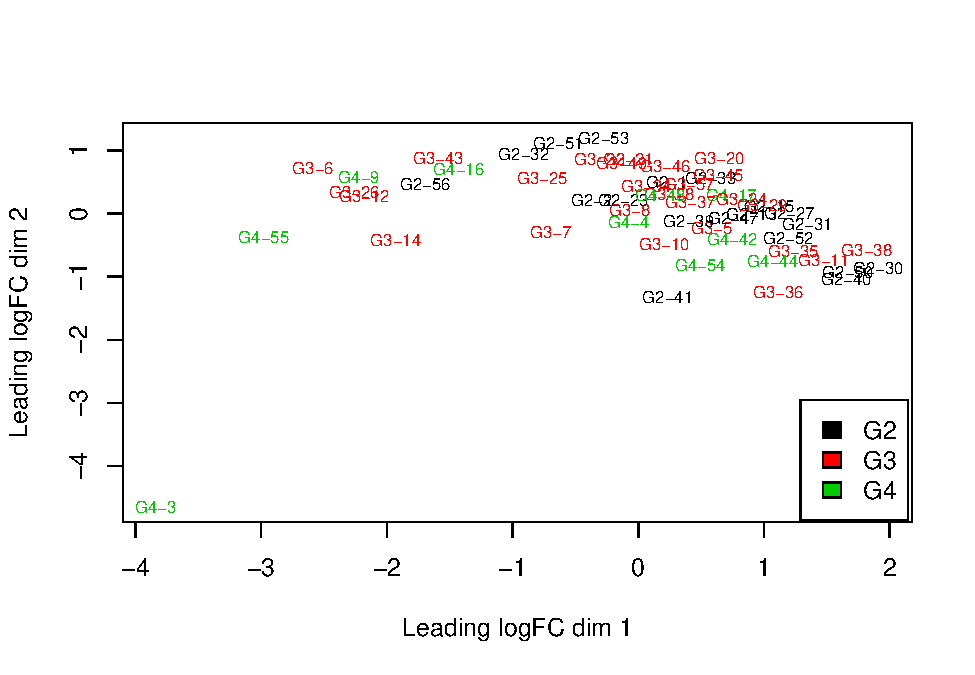
\includegraphics{IEO_project_files/figure-latex/unnamed-chunk-4-3.pdf}

\begin{Shaded}
\begin{Highlighting}[]
\NormalTok{###CANCER laterality}
\NormalTok{tumor_lat_se <-}\StringTok{ }\NormalTok{tumor_se[,!}\KeywordTok{is.na}\NormalTok{(tumor_se$laterality)]}
\NormalTok{tumor_late_dge <-tumor_dge[,!}\KeywordTok{is.na}\NormalTok{(tumor_se$laterality)]}
\NormalTok{batch <-}\StringTok{ }\KeywordTok{as.integer}\NormalTok{(}\KeywordTok{factor}\NormalTok{(tumor_lat_se$laterality))}
\NormalTok{outcome <-}\StringTok{ }\KeywordTok{paste}\NormalTok{(}\KeywordTok{factor}\NormalTok{(tumor_lat_se$laterality), }\KeywordTok{colnames}\NormalTok{(tumor_lat_se), }\DataTypeTok{sep=}\StringTok{"-"}\NormalTok{)}
\KeywordTok{plotMDS}\NormalTok{(tumor_stage_dge, }\DataTypeTok{col =} \NormalTok{batch,}\DataTypeTok{labels =} \NormalTok{outcome, }\DataTypeTok{cex =} \FloatTok{0.7}\NormalTok{)}
\KeywordTok{legend}\NormalTok{(}\StringTok{"topleft"}\NormalTok{, }\KeywordTok{sort}\NormalTok{(}\KeywordTok{unique}\NormalTok{(batch)), }\KeywordTok{levels}\NormalTok{(}\KeywordTok{factor}\NormalTok{(tumor_lat_se$laterality)), }\DataTypeTok{fill=}\KeywordTok{sort}\NormalTok{(}\KeywordTok{unique}\NormalTok{(batch)), }\DataTypeTok{inset=}\FloatTok{0.005}\NormalTok{)}
\end{Highlighting}
\end{Shaded}

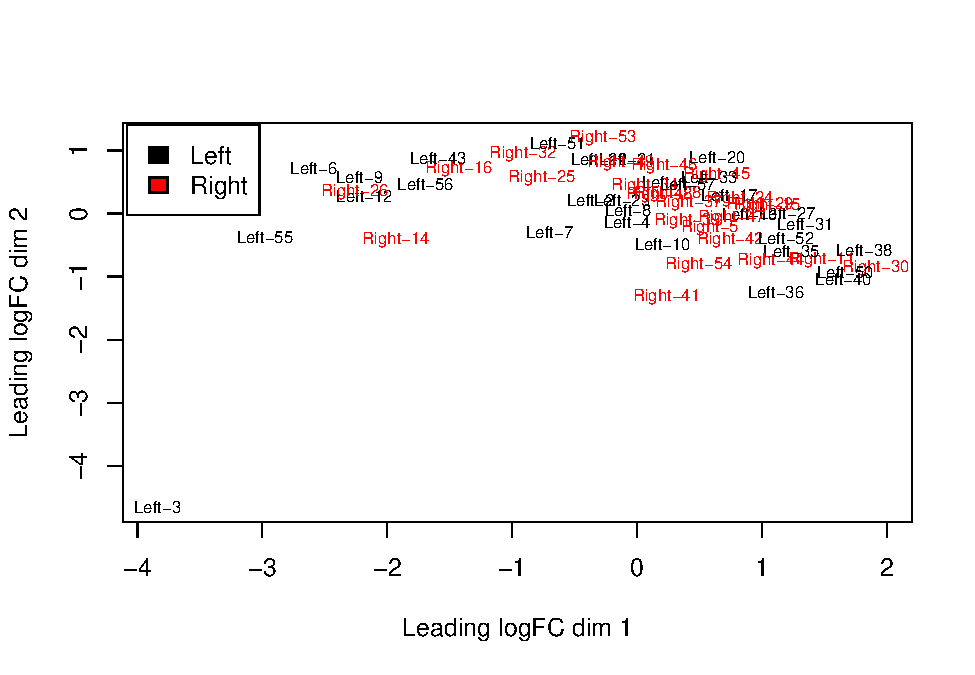
\includegraphics{IEO_project_files/figure-latex/unnamed-chunk-4-4.pdf}

\begin{Shaded}
\begin{Highlighting}[]
\NormalTok{###CANCER status}
\NormalTok{tumor_status_se <-}\StringTok{ }\NormalTok{tumor_se[,!}\KeywordTok{is.na}\NormalTok{(tumor_se$vital_status)]}
\NormalTok{tumor_status_dge <-tumor_dge[,!}\KeywordTok{is.na}\NormalTok{(tumor_se$vital_status)]}
\NormalTok{batch <-}\StringTok{ }\KeywordTok{as.integer}\NormalTok{(}\KeywordTok{factor}\NormalTok{(tumor_status_se$vital_status))}
\NormalTok{outcome <-}\StringTok{ }\KeywordTok{paste}\NormalTok{(}\KeywordTok{factor}\NormalTok{(tumor_status_se$vital_status), }\KeywordTok{colnames}\NormalTok{(tumor_status_se), }\DataTypeTok{sep=}\StringTok{"-"}\NormalTok{)}
\KeywordTok{plotMDS}\NormalTok{(tumor_status_dge, }\DataTypeTok{col =} \NormalTok{batch,}\DataTypeTok{labels =} \NormalTok{outcome, }\DataTypeTok{cex =} \FloatTok{0.7}\NormalTok{)}
\KeywordTok{legend}\NormalTok{(}\StringTok{"topleft"}\NormalTok{, }\KeywordTok{sort}\NormalTok{(}\KeywordTok{unique}\NormalTok{(batch)), }\KeywordTok{levels}\NormalTok{(}\KeywordTok{factor}\NormalTok{(tumor_status_se$vital_status)), }\DataTypeTok{fill=}\KeywordTok{sort}\NormalTok{(}\KeywordTok{unique}\NormalTok{(batch)), }\DataTypeTok{inset=}\FloatTok{0.005}\NormalTok{)}
\end{Highlighting}
\end{Shaded}

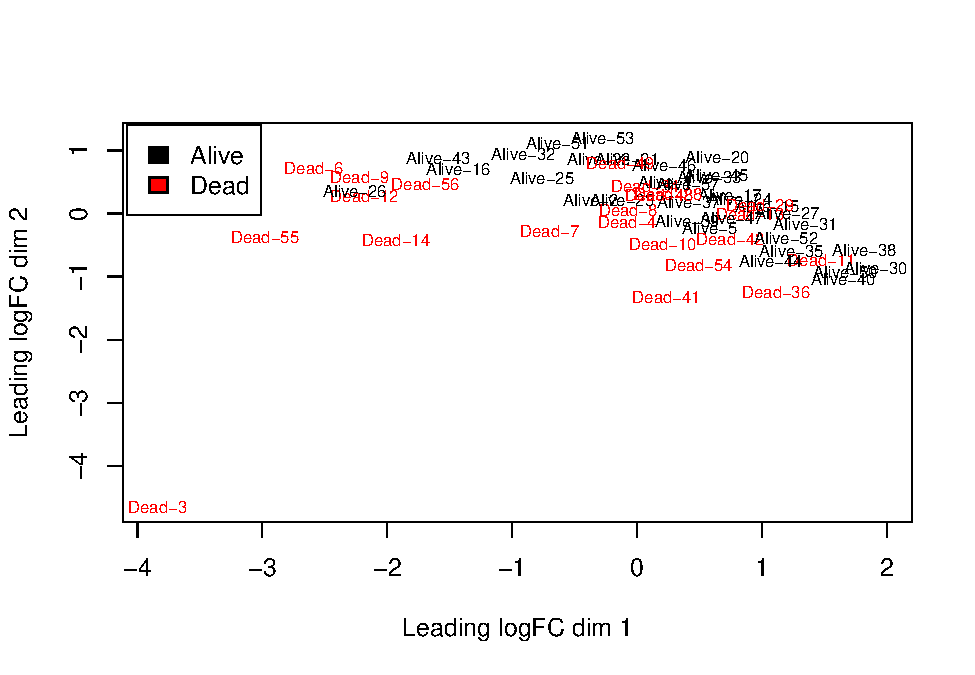
\includegraphics{IEO_project_files/figure-latex/unnamed-chunk-4-5.pdf}

\subsection{3. Differential expression}\label{differential-expression}

\begin{Shaded}
\begin{Highlighting}[]
\KeywordTok{library}\NormalTok{(sva)}
\end{Highlighting}
\end{Shaded}

\begin{verbatim}
## Warning: package 'sva' was built under R version 3.4.2
\end{verbatim}

\begin{verbatim}
## Loading required package: mgcv
\end{verbatim}

\begin{verbatim}
## Loading required package: nlme
\end{verbatim}

\begin{verbatim}
## 
## Attaching package: 'nlme'
\end{verbatim}

\begin{verbatim}
## The following object is masked from 'package:IRanges':
## 
##     collapse
\end{verbatim}

\begin{verbatim}
## This is mgcv 1.8-17. For overview type 'help("mgcv-package")'.
\end{verbatim}

\begin{verbatim}
## Loading required package: genefilter
\end{verbatim}

\begin{verbatim}
## Warning: package 'genefilter' was built under R version 3.4.2
\end{verbatim}

\begin{verbatim}
## 
## Attaching package: 'genefilter'
\end{verbatim}

\begin{verbatim}
## The following objects are masked from 'package:matrixStats':
## 
##     rowSds, rowVars
\end{verbatim}

\begin{verbatim}
## Loading required package: BiocParallel
\end{verbatim}

\begin{verbatim}
## Warning: package 'BiocParallel' was built under R version 3.4.2
\end{verbatim}

\begin{Shaded}
\begin{Highlighting}[]
\NormalTok{mod <-}\StringTok{ }\KeywordTok{model.matrix}\NormalTok{(~}\StringTok{ }\NormalTok{se.filt4$type, }\KeywordTok{colData}\NormalTok{(se.filt4))}
\NormalTok{mod0 <-}\StringTok{ }\KeywordTok{model.matrix}\NormalTok{(~}\StringTok{ }\DecValTok{1}\NormalTok{, }\KeywordTok{colData}\NormalTok{(se.filt4))}
\NormalTok{pv <-}\StringTok{ }\KeywordTok{f.pvalue}\NormalTok{(}\KeywordTok{assays}\NormalTok{(se.filt4)$logCPM, mod, mod0)}
\KeywordTok{sum}\NormalTok{(}\KeywordTok{p.adjust}\NormalTok{(pv, }\DataTypeTok{method=}\StringTok{"fdr"}\NormalTok{)<}\StringTok{ }\FloatTok{0.01}\NormalTok{)}
\end{Highlighting}
\end{Shaded}

\begin{verbatim}
## [1] 10601
\end{verbatim}

\begin{Shaded}
\begin{Highlighting}[]
\KeywordTok{hist}\NormalTok{(pv, }\DataTypeTok{main=}\StringTok{""}\NormalTok{,}\DataTypeTok{las=}\DecValTok{1}\NormalTok{)}
\end{Highlighting}
\end{Shaded}

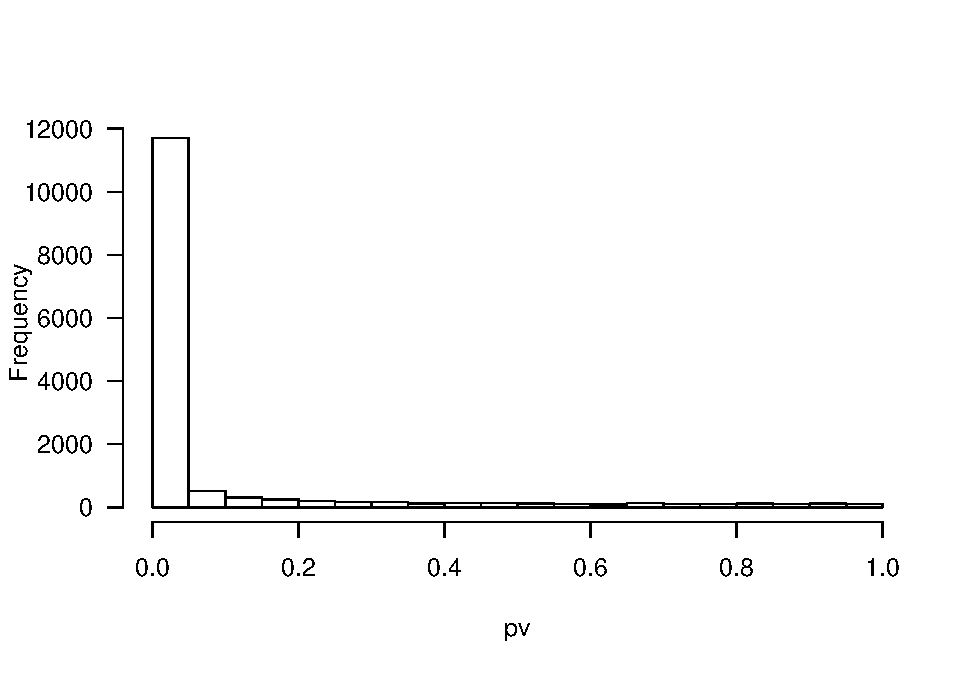
\includegraphics{IEO_project_files/figure-latex/Differential expression-1.pdf}

Estimation of surrogate variables

\begin{Shaded}
\begin{Highlighting}[]
\NormalTok{sv <-}\StringTok{ }\KeywordTok{sva}\NormalTok{(}\KeywordTok{assays}\NormalTok{(se.filt4)$logCPM, mod, mod0)}
\end{Highlighting}
\end{Shaded}

\begin{verbatim}
## Number of significant surrogate variables is:  18 
## Iteration (out of 5 ):1  2  3  4  5
\end{verbatim}

\begin{Shaded}
\begin{Highlighting}[]
\NormalTok{sv$n}
\end{Highlighting}
\end{Shaded}

\begin{verbatim}
## [1] 18
\end{verbatim}

\begin{Shaded}
\begin{Highlighting}[]
\NormalTok{modsv <-}\StringTok{ }\KeywordTok{cbind}\NormalTok{(mod, sv$sv)}
\NormalTok{mod0sv <-}\StringTok{ }\KeywordTok{cbind}\NormalTok{(mod0, sv$sv)}
\NormalTok{pvsv <-}\StringTok{ }\KeywordTok{f.pvalue}\NormalTok{(}\KeywordTok{assays}\NormalTok{(se.filt4)$logCPM, modsv, mod0sv)}
\KeywordTok{sum}\NormalTok{(}\KeywordTok{p.adjust}\NormalTok{(pvsv,}\DataTypeTok{method=}\StringTok{"fdr"}\NormalTok{)<}\FloatTok{0.01}\NormalTok{)}
\end{Highlighting}
\end{Shaded}

\begin{verbatim}
## [1] 11973
\end{verbatim}

\begin{Shaded}
\begin{Highlighting}[]
\KeywordTok{hist}\NormalTok{(pvsv, }\DataTypeTok{main=}\StringTok{""}\NormalTok{,}\DataTypeTok{las=}\DecValTok{1}\NormalTok{)}
\end{Highlighting}
\end{Shaded}

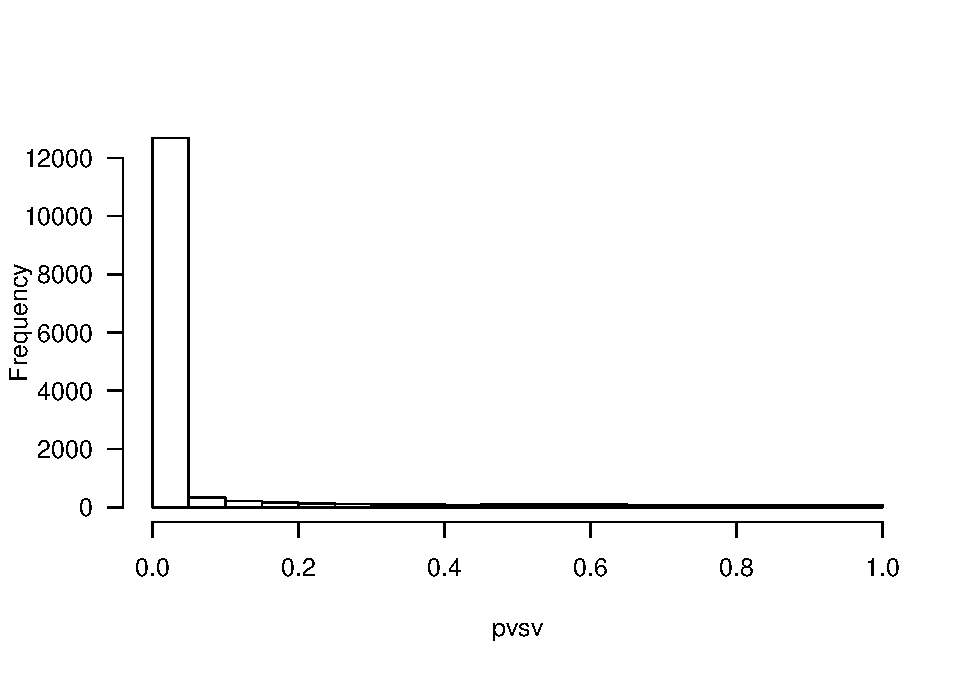
\includegraphics{IEO_project_files/figure-latex/Estimation of surrogate variables-1.pdf}

Fold change

\begin{Shaded}
\begin{Highlighting}[]
\NormalTok{tumorExp <-}\StringTok{ }\KeywordTok{rowMeans}\NormalTok{(logCPM[, se.filt4$type ==}\StringTok{ "tumor"}\NormalTok{])}
\NormalTok{normalExp <-}\StringTok{ }\KeywordTok{rowMeans}\NormalTok{(logCPM[, se.filt4$type ==}\StringTok{ "normal"}\NormalTok{])}
\KeywordTok{par}\NormalTok{(}\DataTypeTok{mfrow =} \KeywordTok{c}\NormalTok{(}\DecValTok{1}\NormalTok{, }\DecValTok{2}\NormalTok{))}
\KeywordTok{plot}\NormalTok{(normalExp, tumorExp, }\DataTypeTok{xlab =} \StringTok{"Tumor"}\NormalTok{, }\DataTypeTok{ylab =} \StringTok{"Normal"}\NormalTok{, }\DataTypeTok{pch =} \StringTok{"."}\NormalTok{, }\DataTypeTok{cex =} \DecValTok{4}\NormalTok{, }\DataTypeTok{las =} \DecValTok{1}\NormalTok{)}
\KeywordTok{plot}\NormalTok{((tumorExp +}\StringTok{ }\NormalTok{normalExp)/}\DecValTok{2}\NormalTok{, tumorExp -}\StringTok{ }\NormalTok{normalExp, }\DataTypeTok{pch =} \StringTok{"."}\NormalTok{, }\DataTypeTok{cex =} \DecValTok{4}\NormalTok{, }\DataTypeTok{las =} \DecValTok{1}\NormalTok{)}
\end{Highlighting}
\end{Shaded}

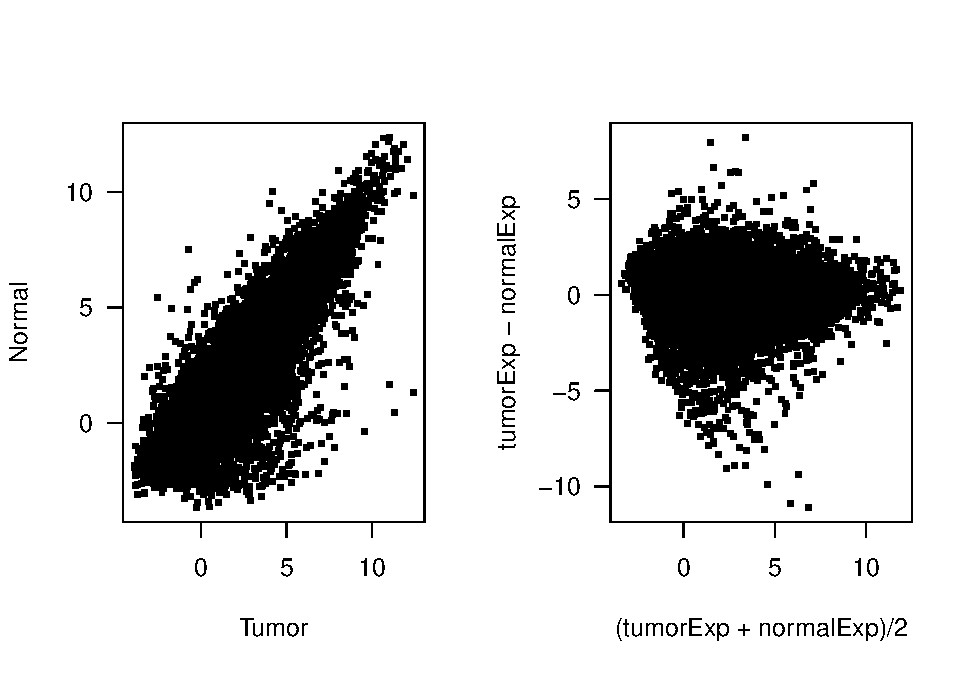
\includegraphics{IEO_project_files/figure-latex/Fold change-1.pdf}

\begin{Shaded}
\begin{Highlighting}[]
\NormalTok{log2fc <-}\StringTok{ }\NormalTok{tumorExp -}\StringTok{ }\NormalTok{normalExp}
\NormalTok{ranking <-}\StringTok{ }\KeywordTok{order}\NormalTok{(}\KeywordTok{abs}\NormalTok{(log2fc), }\DataTypeTok{decreasing =} \OtherTok{TRUE}\NormalTok{)}
\KeywordTok{head}\NormalTok{(}\KeywordTok{data.frame}\NormalTok{(}\DataTypeTok{Log2FC =} \KeywordTok{round}\NormalTok{(log2fc[ranking], }\DataTypeTok{digits =} \DecValTok{3}\NormalTok{), }\DataTypeTok{FC =} \KeywordTok{round}\NormalTok{(}\DecValTok{2}\NormalTok{^log2fc[ranking], }
    \DataTypeTok{digits =} \DecValTok{3}\NormalTok{), }\StringTok{`}\DataTypeTok{1/FC}\StringTok{`} \NormalTok{=}\StringTok{ }\KeywordTok{round}\NormalTok{(}\DecValTok{2}\NormalTok{^(-log2fc[ranking]), }\DataTypeTok{digits =} \DecValTok{3}\NormalTok{), }\DataTypeTok{row.names =} \KeywordTok{rowData}\NormalTok{(se.filt4)$symbol[ranking], }
    \DataTypeTok{check.names =} \OtherTok{FALSE}\NormalTok{), }\DataTypeTok{n =} \DecValTok{10}\NormalTok{)}
\end{Highlighting}
\end{Shaded}

\begin{verbatim}
##          Log2FC      FC     1/FC
## ZNF880  -11.083   0.000 2169.764
## AQP4    -10.886   0.001 1892.719
## LAMTOR3  -9.910   0.001  962.404
## SRP54    -9.358   0.002  656.130
## CLDND2   -9.069   0.002  537.101
## GALT     -8.916   0.002  482.951
## WDFY2    -8.907   0.002  480.171
## OR2M7    -8.337   0.003  323.423
## CAB39L    8.202 294.522    0.003
## ATP6V0C  -8.105   0.004  275.302
\end{verbatim}


\end{document}
